% ------------------------------------------------------ %
% 由于很多参加数学建模竞赛的同学没有\LaTeX基础,因此做
% 本模板用于各位写手快速上手写作,不要追究原理,先把模
% 板用会再说
% ------------------------------------------------------ %
%         谈欣 如有错误请联系1792733991@qq.com
%         谈欣 如有错误请联系1792733991@qq.com
%         谈欣 如有错误请联系1792733991@qq.com
% ------------------------------------------------------ %
%     更多内容关注:
%     个人网页:https://jack-tanxin.github.io
%     个人Github主页:https://github.com/Jack-TanXin
% ------------------------------------------------------ %
% 数学建模论文是个结构非常复杂的论文,因此使用\LaTeX必须
% 编译数次——无论你使用哪种发行版或编辑器,原因详见\LaTeX
% 的编译原理,一般写好以后编译2次就是文章真正的面目。
% ------------------------------------------------------ %
\documentclass[UTF8,12pt]{ctexart}

% ------------------------------------------------------ %
% 下面的包基本上都是数学建模必需的包,没有这些包我想基
% 本上是写不出完整的论文的,仅供大家参考
% ------------------------------------------------------ %
\usepackage[a4paper,left=2.5cm,right=2.5cm,top=2.5cm,bottom=2.5cm]{geometry}    % 这个包专门用来调整页边距
\usepackage{amsmath}    % 数学包
\usepackage{fancyhdr}   % 页眉页脚设定

% 插入图片的包
\usepackage{graphicx}
\usepackage{subfigure}

% 表格包
\usepackage{float}
\usepackage{booktabs}



% 务必注意:图片在figures目录下
% 务必注意:图片在figures目录下
% 务必注意:图片在figures目录下
\graphicspath{{figures/}} 



\begin{document}   % 文章开始



% ----------------------------------------------- %
%              请在这里输入文章标题
% ----------------------------------------------- %
%              请在这里输入文章标题
% ----------------------------------------------- %
\title{基于树的玻璃文物的成分分析与鉴别}



\author{} % 不要动
\date{} % 不要动
\maketitle % 不要动
\vspace{-4em}  % 消除作者和日期造成的空白



% ---------------------------------------------------- %
%  打开chapter文件夹里的摘要.tex文件,编辑其中的内容
% ---------------------------------------------------- %
%  打开chapter文件夹里的摘要.tex文件,编辑其中的内容
% ---------------------------------------------------- %
\begin{abstract}

    一句话概括整个赛题的要求和你要怎么思考,总之这里就是一个很大的话~
    
    \textbf{针对问题一:}摘要内容摘要内容摘要内容摘要内容摘要内容摘要内容摘要内容摘要内容摘要内容摘要内容摘要内容摘要内容摘要内容摘要内容摘要内容摘要内容摘要内容摘要内容摘要内容摘要内容摘要内容摘要内容摘要内容摘要内容摘要内容摘要内容摘要内容摘要内容摘要内容摘要内容摘要内容摘要内容摘要内容摘要内容摘要内容摘要内容摘要内容摘要内容摘要内容摘要内容摘要内容摘要内容摘要内容。
    
    \textbf{针对问题二:}摘要内容摘要内容摘要内容摘要内容摘要内容摘要内容摘要内容摘要内容摘要内容摘要内容摘要内容摘要内容摘要内容摘要内容摘要内容摘要内容摘要内容摘要内容摘要内容摘要内容摘要内容摘要内容摘要内容摘要内容摘要内容摘要内容摘要内容摘要内容摘要内容摘要内容摘要内容摘要内容摘要内容摘要内容摘要内容摘要内容摘要内容摘要内容摘要内容摘要内容摘要内容摘要内容摘要内容。
    
    \textbf{针对问题三:}摘要内容摘要内容摘要内容摘要内容摘要内容摘要内容摘要内容摘要内容摘要内容摘要内容摘要内容摘要内容摘要内容摘要内容摘要内容摘要内容摘要内容摘要内容摘要内容摘要内容摘要内容摘要内容摘要内容摘要内容摘要内容摘要内容摘要内容摘要内容摘要内容摘要内容摘要内容摘要内容摘要内容摘要内容摘要内容摘要内容摘要内容摘要内容摘要内容摘要内容摘要内容摘要内容摘要内容。
    
    \textbf{针对问题四:}摘要内容摘要内容摘要内容摘要内容摘要内容摘要内容摘要内容摘要内容摘要内容摘要内容摘要内容摘要内容摘要内容摘要内容摘要内容摘要内容摘要内容摘要内容摘要内容摘要内容摘要内容摘要内容摘要内容摘要内容摘要内容摘要内容摘要内容摘要内容摘要内容摘要内容摘要内容摘要内容摘要内容摘要内容摘要内容摘要内容摘要内容摘要内容摘要内容摘要内容摘要内容摘要内容摘要内容。
    
    \vspace{1em} % 移除2个行距的空白:这句代码千万不能动!!!移除2个行距的空白:这句代码千万不能动!!!
    
    \noindent{\textbf{关键词:}随机森林;方差选择法;Voting Classifier;层次聚类分析;决策树}
    
\end{abstract} 



\thispagestyle{empty}  % 清除摘要页的页码
\newpage  % 另开一页写目录



% ------------------------------------------------------------ %
%    这一部分自动生成目录,同时清除目录页的页眉和页脚,
%    清除目录页的页码以保证正文的第一面为页码1
%    并新开一面
% ------------------------------------------------------------ %
\pagestyle{fancy}
\fancyhead{} % 页眉清空
\fancyfoot{} % 页脚清空
\begin{center} \tableofcontents \end{center}
\thispagestyle{empty}\newpage



% ------------------------------------------------------------ %
%    设置正文的页眉、页脚,页眉没有内容,页码在页脚中间
%    并将本页设置为第一页
% ------------------------------------------------------------ %
\pagestyle{fancy}
\fancyhead[R]{} % 页眉右侧清空
\fancyhead[C]{} % 页眉中间清空
\fancyhead[L]{} % 页眉左侧清空
\fancyfoot[R]{} % 页脚右侧清空
\fancyfoot[C]{- {\thepage}\ -} % 页脚中间为页码
\fancyfoot[L]{} % 页脚左侧清空
\setcounter{page}{1}  



% ---------------------------------------------------------- %
% 接下来的部分即为文章每个章节的内容,我这里使用的是2022年
% 国赛的论文,当时是有四道题目,每次竞赛的题目量都不一定,
% 请酌情更改,另外有时候可能会多一个灵敏度分析或是其他创新
% 的内容,记住一个准则:有多少个章节就在chapter文件夹中制作
% 多少个tex文件,每个文件夹管一个章节就行啦!!!
% ---------------------------------------------------------- %



% ---------------------------------------------------------- %
%    打开chapter文件夹里的问题重述.tex文件,编辑其中的内容
% ---------------------------------------------------------- %
%    打开chapter文件夹里的问题重述.tex文件,编辑其中的内容
% ---------------------------------------------------------- %
\section{问题重述}

\subsection{问题背景}

问题背景内容问题背景内容问题背景内容问题背景内容问题背景内容问题背景内容问题背景内容问题背景内容问题背景内容问题背景内容问题背景内容问题背景内容问题背景内容问题背景内容问题背景内容问题背景内容问题背景内容问题背景内容问题背景内容问题背景内容问题背景内容问题背景内容问题背景内容问题背景内容问题背景内容问题背景内容问题背景内容问题背景内容问题背景内容问题背景内容问题背景内容问题背景内容问题背景内容问题背景内容问题背景内容问题背景内容问题背景内容问题背景内容问题背景内容问题背景内容问题背景内容问题背景内容问题背景内容问题背景内容问题背景内容问题背景内容

\subsection{问题提出}

现有一组由专家给出的关于玻璃的数据,要求通过分析与建模解决下面若干问题:

\textbf{问题1} 问题提出内容问题提出内容问题提出内容问题提出内容问题提出内容问题提出内容问题提出内容问题提出内容。

\textbf{问题2} 问题提出内容问题提出内容问题提出内容问题提出内容问题提出内容问题提出内容问题提出内容问题提出内容问题提出内容。

\textbf{问题3} 问题提出内容问题提出内容问题提出内容问题提出内容问题提出内容问题提出内容问题提出内容问题提出内容问题提出内容。

\textbf{问题4} 问题提出内容问题提出内容问题提出内容问题提出内容问题提出内容问题提出内容问题提出内容问题提出内容问题提出内容。



% ---------------------------------------------------------- %
%    打开chapter文件夹里的问题分析.tex文件,编辑其中的内容
% ---------------------------------------------------------- %
%    打开chapter文件夹里的问题分析.tex文件,编辑其中的内容
% ---------------------------------------------------------- %
\section{问题分析}

\subsection{问题一的分析}

问题分析内容问题分析内容问题分析内容问题分析内容问题分析内容问题分析内容问题分析内容问题分析内容问题分析内容问题分析内容问题分析内容问题分析内容问题分析内容问题分析内容问题分析内容问题分析内容问题分析内容问题分析内容问题分析内容问题分析内容问题分析内容问题分析内容问题分析内容问题分析内容问题分析内容问题分析内容问题分析内容问题分析内容问题分析内容问题分析内容问题分析内容

问题分析内容问题分析内容问题分析内容问题分析内容问题分析内容问题分析内容问题分析内容问题分析内容问题分析内容问题分析内容问题分析内容问题分析内容问题分析内容问题分析内容问题分析内容问题分析内容问题分析内容问题分析内容问题分析内容问题分析内容问题分析内容问题分析内容问题分析内容问题分析内容问题分析内容问题分析内容问题分析内容问题分析内容问题分析内容

\subsection{问题二的分析}

问题分析内容问题分析内容问题分析内容问题分析内容问题分析内容问题分析内容问题分析内容问题分析内容问题分析内容问题分析内容问题分析内容问题分析内容问题分析内容问题分析内容问题分析内容问题分析内容问题分析内容问题分析内容问题分析内容问题分析内容问题分析内容问题分析内容问题分析内容问题分析内容问题分析内容问题分析内容问题分析内容问题分析内容问题分析内容问题分析内容问题分析内容

问题分析内容问题分析内容问题分析内容问题分析内容问题分析内容问题分析内容问题分析内容问题分析内容问题分析内容问题分析内容问题分析内容问题分析内容问题分析内容问题分析内容问题分析内容问题分析内容问题分析内容问题分析内容问题分析内容问题分析内容问题分析内容问题分析内容问题分析内容问题分析内容问题分析内容问题分析内容问题分析内容问题分析内容问题分析内容

\subsection{问题三的分析}

问题分析内容问题分析内容问题分析内容问题分析内容问题分析内容问题分析内容问题分析内容问题分析内容问题分析内容问题分析内容问题分析内容问题分析内容问题分析内容问题分析内容问题分析内容问题分析内容问题分析内容问题分析内容问题分析内容问题分析内容问题分析内容问题分析内容问题分析内容问题分析内容问题分析内容问题分析内容问题分析内容问题分析内容问题分析内容问题分析内容问题分析内容

问题分析内容问题分析内容问题分析内容问题分析内容问题分析内容问题分析内容问题分析内容问题分析内容问题分析内容问题分析内容问题分析内容问题分析内容问题分析内容问题分析内容问题分析内容问题分析内容问题分析内容问题分析内容问题分析内容问题分析内容问题分析内容问题分析内容问题分析内容问题分析内容问题分析内容问题分析内容问题分析内容问题分析内容问题分析内容

\subsection{问题四的分析}

问题分析内容问题分析内容问题分析内容问题分析内容问题分析内容问题分析内容问题分析内容问题分析内容问题分析内容问题分析内容问题分析内容问题分析内容问题分析内容问题分析内容问题分析内容问题分析内容问题分析内容问题分析内容问题分析内容问题分析内容问题分析内容问题分析内容问题分析内容问题分析内容问题分析内容问题分析内容问题分析内容问题分析内容问题分析内容问题分析内容问题分析内容

问题分析内容问题分析内容问题分析内容问题分析内容问题分析内容问题分析内容问题分析内容问题分析内容问题分析内容问题分析内容问题分析内容问题分析内容问题分析内容问题分析内容问题分析内容问题分析内容问题分析内容问题分析内容问题分析内容问题分析内容问题分析内容问题分析内容问题分析内容问题分析内容问题分析内容问题分析内容问题分析内容问题分析内容问题分析内容




% ---------------------------------------------------------- %
%    打开chapter文件夹里的模型假设.tex文件,编辑其中的内容
% ---------------------------------------------------------- %
%    打开chapter文件夹里的模型假设.tex文件,编辑其中的内容
% ---------------------------------------------------------- %
\section{模型假设}

\noindent{1.假设所给数据真实可靠。}

\noindent{2.本文认为在对样本进行采样过程中没有破坏样本的完整性。}

\noindent{3.玻璃统计规律可以代表玻璃的一般规律,不随其他无关因素而改变。}

\noindent{4.从玻璃内部的所取化学物质与表中所给物质吻合,不发生化学反应。}

\noindent{5.针对不同玻璃,其颜色特征不会因光照等因素而发生改变。}

\noindent{6.针对不同的化学成分,在风化前后的化学物质的比例稳定。}

\noindent{7.化学成分含量发生变化也适用于变化前的模型规律。}



% ---------------------------------------------------------- %
%    打开chapter文件夹里的符号说明.tex文件,编辑其中的内容
% ---------------------------------------------------------- %
%    打开chapter文件夹里的符号说明.tex文件,编辑其中的内容
% ---------------------------------------------------------- %
\section{符号说明}


\begin{table}[H]
	\centering
	\begin{tabular}{c c} 
		\toprule[1.5pt]
		符号 & 含义  \\ 
		\midrule[1pt]
		$i=1,i=2$ & 分别表示高钾、铅钡玻璃 \\ 
		$j$ & 表示表中从二氧化硅($SiO_2$)到二氧化硫($SO_2$)中第$j$类化学物质 \\
		$z=1,z=2$ & 分别表示风化前和风化后 \\
		$x_1,x_2,x_3,x_4$ & 分别表示纹饰、类型、颜色、风化表面 \\
		$y_j$ & 表示第$j$类化学物质的含量 \\ 
		$\overline{y_j}$ & 表示第$j$类化学物质的平均含量 \\  
		\toprule[1.5pt]
	\end{tabular}
\end{table}



% ------------------------------------------------------------ %
%    打开chapter文件夹里的问题一建模.tex文件,编辑其中的内容
% ------------------------------------------------------------ %
%    打开chapter文件夹里的问题一建模.tex文件,编辑其中的内容
% ------------------------------------------------------------ %
\section{问题一建模与求解}

为分析玻璃文物的表面风化与其玻璃类型、纹饰和颜色的关系以及文物样品表面有无风化化学成分含量的统计规律,并对风化前的化学含量进行分析,制作流程图如下:

\begin{figure}[H] 
	\centering %图片居中
	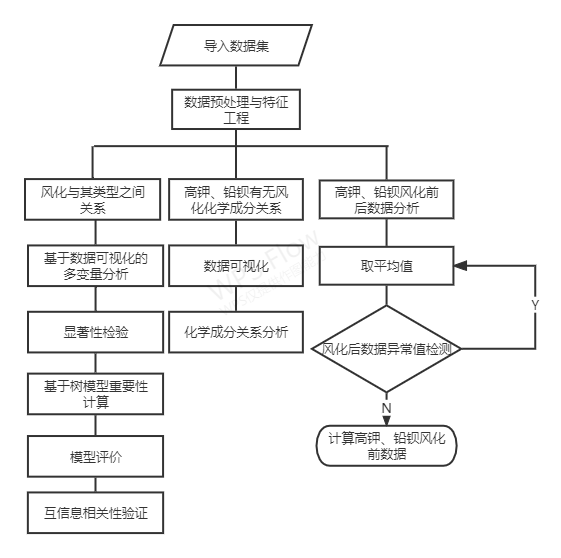
\includegraphics[width=0.7\textwidth]{1.png} %插入图片,[]中设置图片大小,{}中是图片文件名
	\caption{问题一流程图} %最终文档中希望显示的图片标题
	\label{Fig.main2} %用于文内引用的标签
\end{figure}

\subsection{模型准备——数据预处理与特征工程}

\subsubsection{数据清洗}

本文根据附件表1所给的数据,通过Pandas库进行数据读取,使用isnull函数查找数据中的缺失值,由此发现颜色特征中有数个缺失值,由数据可视化发现黑色文物必定被风化,而缺失值所在样本均为被风化对象,故采用黑色来补全缺失值。

对于附件表2所给的数据,表中空白部分为未检测到的成分将被Pandas视为缺失值,本文指定数值0填补空缺的值以避免缺失值对分析的干扰。

按照题意对其每一行进行求和,选取成分累加和介于85\% ~ 105\%的有效数据并删除不在有效数据范围内的第15个和第17个样品采样点的样本构成新的数据集用于分析。

\subsubsection{特征编码}

为更准确的判断风化情况与三个变量相关关系,依据表1所给的纹饰、类型、颜色以及表面是否风化四个特征对其用特征编码进行分类,由于各个类别之间是相互独立的,故采用独热编码进行特征变换以消除编码后各个类别的不同取值差异对模型训练效果的影响。

然而事与愿违,颜色特征中有七个非序数类别,而独热编码最大的缺点即容易造成编码后数据集的“高维危机”,由此针对颜色特征本文放弃了进行独热编码,而是对其特征编码。

\subsection{玻璃风化与其分类信息关系的分析模型}

\subsubsection{基于数据可视化的多变量分析}

本问要求分析玻璃纹饰、类型、颜色与表面风化情况的关系,基于多变量分析的数据可视化容易分别得到这三个分类特征与风化情况之间的关系,通过Pandas库中的crosstab函数可以实现分类特征之间的多变量分析,图形呈现如下:

\begin{figure}[H] 
	\centering %图片居中
	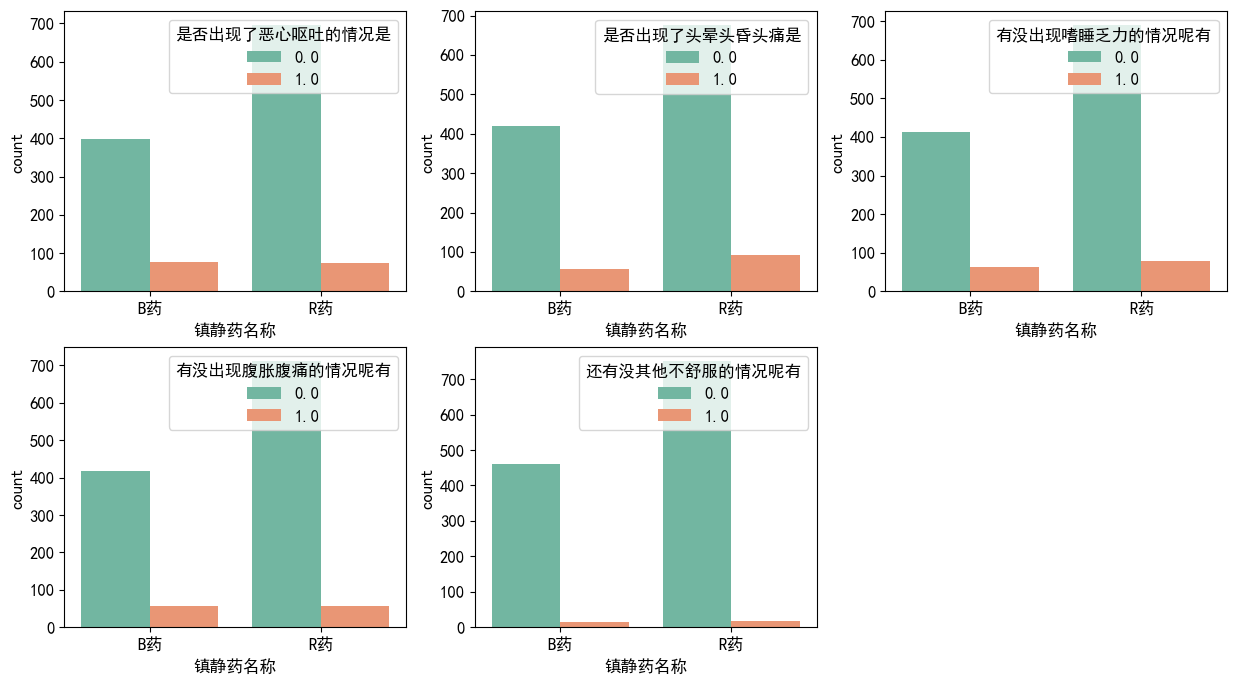
\includegraphics[width=0.7\textwidth]{2.png} %插入图片,[]中设置图片大小,{}中是图片文件名
	\caption{玻璃纹饰与风化情况关系} %最终文档中希望显示的图片标题
	\label{Fig.main3} %用于文内引用的标签
\end{figure}

由图2可知所提供的文物样品中A种纹饰的玻璃中近一半被风化,C种纹饰中风化的玻璃超过一半,而B种纹饰的玻璃全部风化——由此可以推断B类的纹饰与风化情况有极大联系。
下面再来考察玻璃类型与风化情况的关系:

\begin{figure}[H] 
	\centering %图片居中
	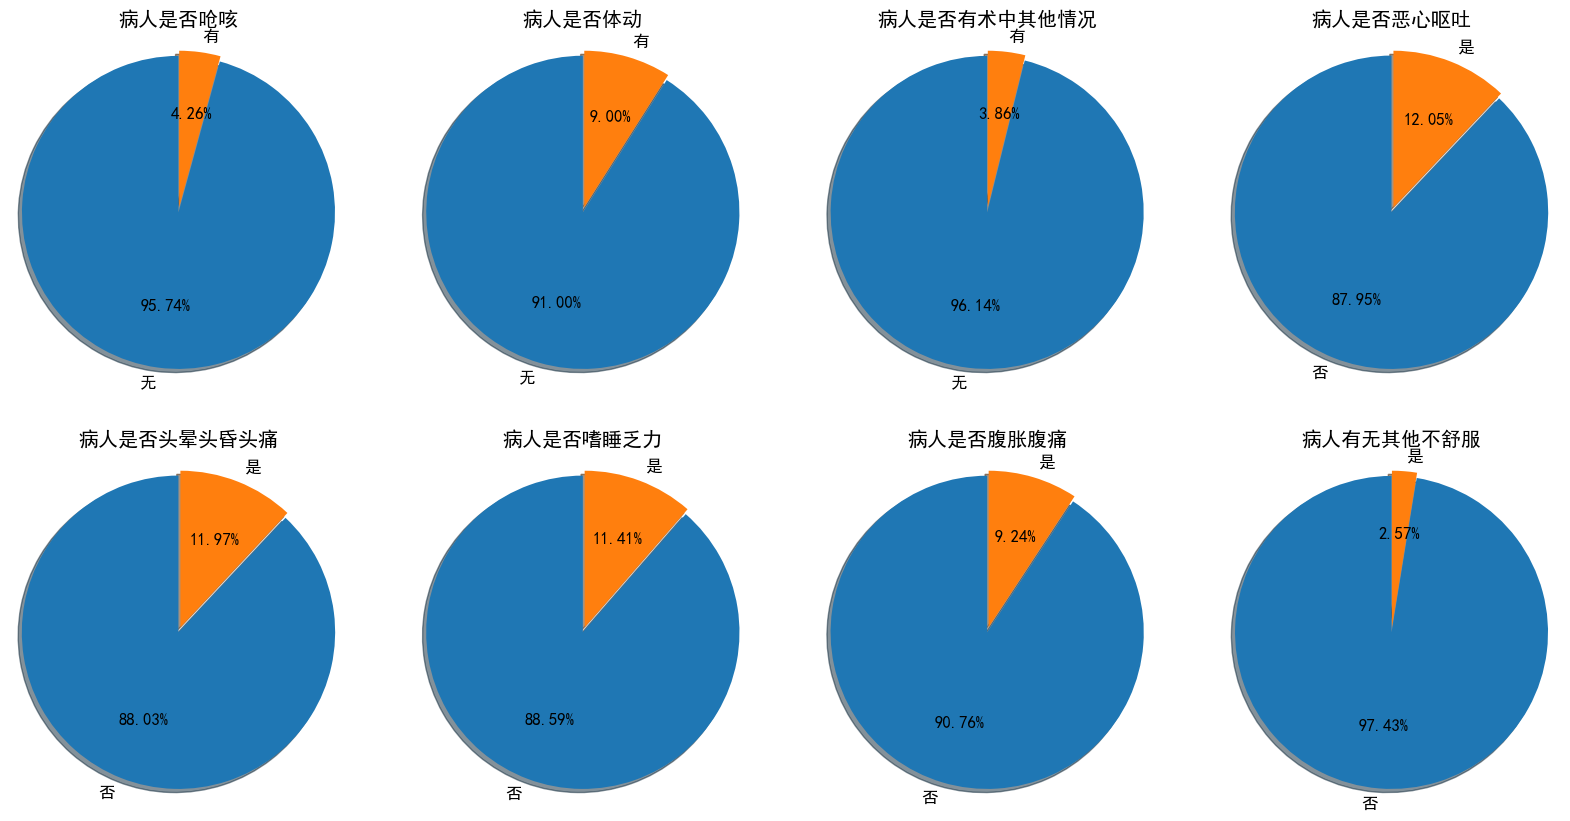
\includegraphics[width=0.7\textwidth]{3.png} %插入图片,[]中设置图片大小,{}中是图片文件名
	\caption{玻璃类型与风化情况关系} %最终文档中希望显示的图片标题
	\label{Fig.main4} %用于文内引用的标签
\end{figure}

由图3可知,对于样本所给的玻璃类型中高钾类玻璃风化的情况仅占百分之三十五,说明高钾类玻璃被风化的概率较小,而对于铅钡类的玻璃则是达到了百分之七十的风化比例。由此可见铅钡类玻璃更容易被风化。

\begin{figure}[H] 
	\centering %图片居中
	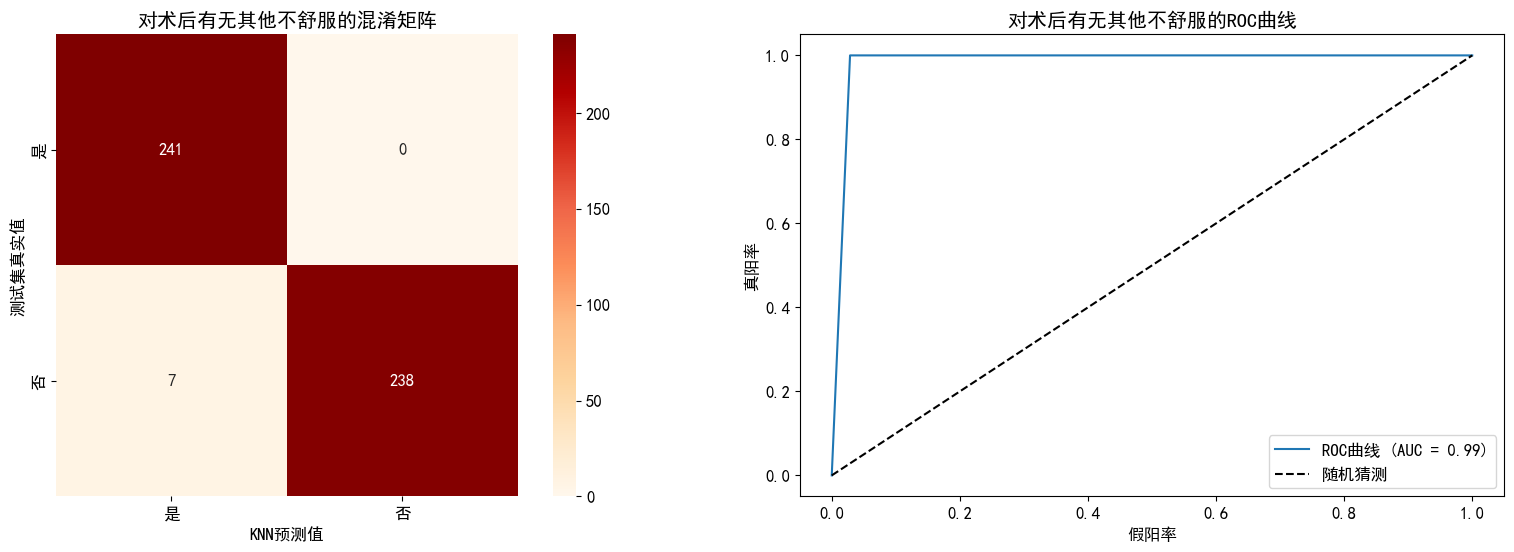
\includegraphics[width=0.7\textwidth]{4.png} %插入图片,[]中设置图片大小,{}中是图片文件名
	\caption{玻璃颜色与风化情况关系} %最终文档中希望显示的图片标题
	\label{Fig.main5} %用于文内引用的标签
\end{figure}

由图4可得,黑色的玻璃样本表面均被风化,而绿色和深蓝色的玻璃样本表面均为未被风化,其余颜色的样本表面被部分风化——由此可见黑色、绿色和深蓝色的玻璃与风化情况存在很大的关系,其他特征无法确定。

综上所述,可以总结出以下规律:

单个分类变量中玻璃纹饰和颜色都存在与表面风化情况确切相关的特征(如B种纹饰必定被风化,黑色文物必定风化,而深蓝和绿色文物均未被风化),而玻璃类型只能得到与风化情况的不同的频率,但不能确定是否风化,因此可以确定纹饰与颜色对玻璃风化的关系紧密,而玻璃类型可能相关性较弱。

下面通过集成学习中的树模型直接说明三种分类变量与玻璃风化情况的强弱关系。

\subsubsection{基于树的模型重要性计算}

通过模型准备中的特征工程本文已经实现了对数据分类特征的编码,经过模型准备的数据可以正式代入随机森林模型进行训练。

树模型作为一种集成学习算法,是一种效果优良的机器学习模型,且其独特的计算特征重要性的功能对于探索本问中多个变量的相关关系具用重要意义。本文基于树模型中最简单的Bagging算法——随机森林,对纹饰、类型、颜色与表面风化情况之间的关系进行分析,具体方法如下:

1. 为消除各类别之间的影响,便于对指标进行比较分析把分类特征编码数据标准化:进行标准化处理

\begin{equation}
  {{z}_{i}}=\frac{{{x}_{i}}-\overline{{{x}_{i}}}}{{{\sigma }_{i}}}
\end{equation}


2. 为找到最优模型,必须对树模型内部参数进行调整,找到最优参数,下面对最优参数进行探究。

(1)训练集的占比直接关系到模型的优劣,寻找训练集与测试集的占比最优参数,让模型达到较好的效果,利用scikit-learn库中的learning curve函数进行训练,并做交叉验证取平均值得到学习曲线图像如下:

\begin{figure}[H] 
	\centering %图片居中
	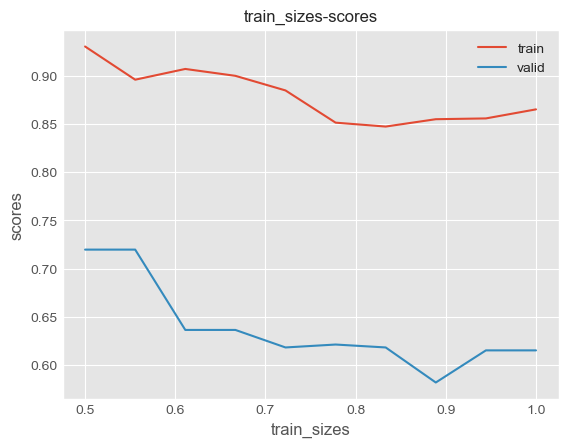
\includegraphics[width=0.7\textwidth]{5.png} %插入图片,[]中设置图片大小,{}中是图片文件名
	\caption{学习曲线} %最终文档中希望显示的图片标题
	\label{Fig.main6} %用于文内引用的标签
\end{figure}


图5可知,训练集占比0.5时,测试集效果最好,因此设置训练集占比为0.55是为最优训练集占比参数。

(2)对于树模型而言,大多数情况下其基学习器的数量是影响其性能的最重要的参数。通过GridSearchCV函数对随机森林模型中决策树的数量进行调整。结果如下:

\begin{figure}[H] 
	\centering %图片居中
	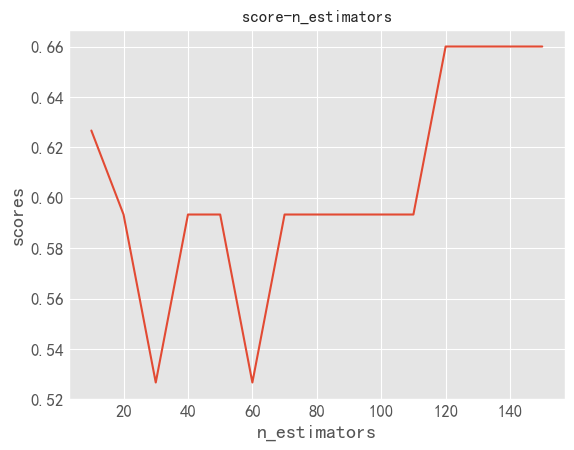
\includegraphics[width=0.7\textwidth]{6.png} %插入图片,[]中设置图片大小,{}中是图片文件名
	\caption{决策树数量图} %最终文档中希望显示的图片标题
	\label{Fig.main7} %用于文内引用的标签
\end{figure}

由图6知,在决策树的数量为120时,模型得分已经达到峰值,此时可以确定决策树的数量最佳值为120。

利用此模型对纹饰、类型、颜色三个特征进行特征重要性计算,结果如下:

\begin{table}[H]
	\centering
	\begin{tabular}{c c c c c c c} 
        \toprule[1.5pt]
		变量 & 纹饰A & 纹饰B & 纹饰C & 高钾类型 & 铅钡类型 & 颜色 \\ 
	    \midrule[1pt]
		评分 & 0.0963 & 0.1014 & 0.0518 & 0.1708 & 0.1809 & 0.3987 \\
        \toprule[1.5pt]
	\end{tabular}
\caption{评分表}
\end{table}



由表1可以看出玻璃纹饰C,纹饰A,纹饰B的评分低,玻璃类型次之,玻璃颜色最大;故本问得出玻璃颜色与玻璃表面风化的关系最强,玻璃的类型次之,而玻璃纹饰与玻璃表面风化关系最弱。结果表示与单个变量重要性之间有所差别,下面进一步说明树模型结果的可靠性以及两种结果差别的原因。

\subsubsection{模型评价}

树模型在本问中能够得到的结果是否可信,需要进一步对模型进行评价。通常是主要通过热力图和ROC图进行判断,同时利用准确率(0.78),精确率,召回率,F1分数,支持率来综合判断模型。根据以上得到的模型参数利用python对模型进行调参后形成新的模型,得到热力图并绘制了ROC曲线测试模型,如下图所示:


\begin{figure}[H] 
	\centering %图片居中
	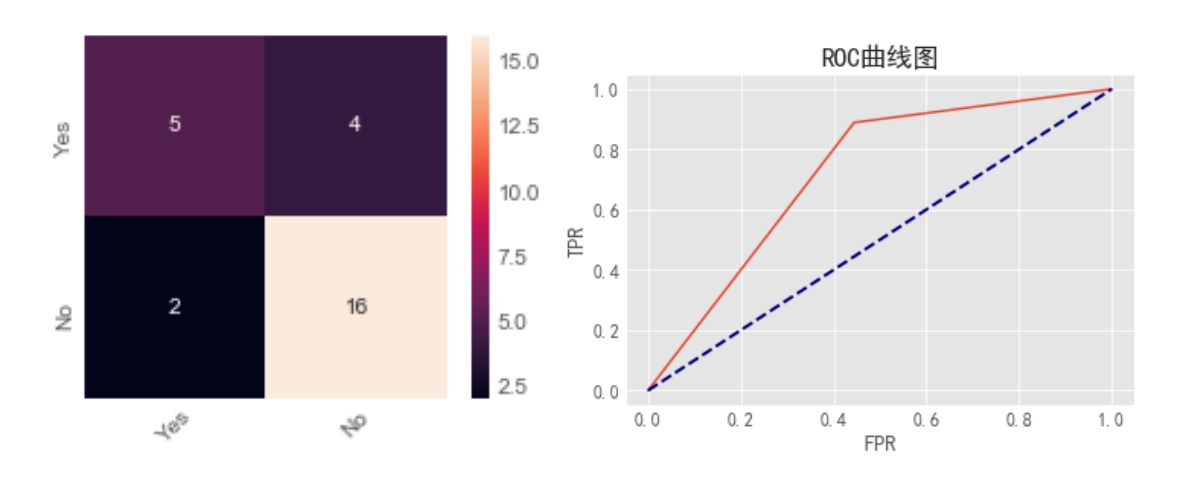
\includegraphics[width=0.7\textwidth]{7.png} %插入图片,[]中设置图片大小,{}中是图片文件名
	\caption{分类结果混淆矩阵热力图} %最终文档中希望显示的图片标题
	\label{Fig.main8} %用于文内引用的标签
\end{figure}

由图7可知,通过热力图知该模型中正确判断未风化的比例占8/9,正确判断风化的比列占5/9;ROC曲线图中可看出此模型的分类器性能极佳,由此认为这个模型可以用来分析批判纹饰、类型、颜色及风化表面之间关系。

对于分类模型的评价还有很多基于混淆矩阵的方法,结合对测试集的预测结果和测试集自身标签、通过计算得到模型的精确度得到如下指标:
\begin{table}[H]
	\centering
	\begin{tabular}{c c c c c} 
		\toprule[1.5pt]
			 & 精确度 & 召回率 & F1分数 & 支持率 \\ 
		\midrule[1pt]
		铅钡 &	0.71 &	0.56 &	0.63 &	9 \\
		高钾 & 	0.80 &	0.89 &	0.84 &	18 \\
		加权平均 &	0.77 &	0.78 &	0.77 &	27 \\
		\toprule[1.5pt]
	\end{tabular}
	\caption{评分数据表}
\end{table}


由表2可知,利用该模型对玻璃类型中高钾和铅钡检验得到的精确度均大于百分之七十,召回率均大于百分之五十,其中高钾类召回率高达百分之八十九,由此可知该模型极为可信,说明该模型对于三种特征的特征重要性评分具有可信度。对于上面结果的不完全相同,可能由于单变量特征重要性没有量化评判标准,导致结果有部分不同,但颜色特征关联最大的特征是确定的,下面对于不同特征重要性进行验证。


\subsubsection{互信息验证}

寻找特征与标签的关系的手段并不是单一的,针对本题数据的具体情况,由于特征和标签均为分类型变量,本文也通过计算互信息以衡量特征与标签间的独立性来验证此题结果。

利用互信息计算风化表面与纹饰,类型,颜色的互信息进一步验证每种关联性的科学性,公式如下:

\begin{equation}
    {{I}_{i}}\left( {{x}_{i}};{{x}_{4}} \right)=\displaystyle\sum\nolimits_{{{x}_{i}},{{x}_{4}}}{p({{x}_{i}},{{x}_{4}})}\log \frac{p({{x}_{i}},{{x}_{4}})}{p({{x}_{i}})p({{x}_{4}})}
\end{equation}

得到互信息表如下: 

\begin{table}[H]
	\centering
	\begin{tabular}{c c c c c} 
	    \toprule[1.5pt]
		& 纹饰 &	类型 &	颜色 &	表面风化情况 \\ 
		\midrule[1pt]
		纹饰 & 	0.943384 &	0.138290 & 	0.383740 &	0.061379 \\
		\hline
		类型 &	0.138290 &	0.619376 &	0.230124 &	0.059385 \\
		\hline
		颜色 &	0.383740 &	0.230124 &	1.609943 &	0.077623 \\
		\hline
		表面风化情况 &	0.061379 &	0.059385 &	0.077623 &	0.678209 \\
	    \toprule[1.5pt]
	\end{tabular}
\caption{互信息表}
\end{table}


由表3知由于纹饰和类型与玻璃表面风化情况的相关性值相差不大(约为0.02),可忽略不计,造成在多个变量共同作用时,类型的占比增大,因此类型的评分增大;而颜色与表面风化情况的相关性评分比其余两个都强,故认为颜色与玻璃文物表面风化有很大联系;此结果与上述模型结果显示一致,由此认为树模型是一个较好的模型且适用于玻璃风化与不同特征重要性评价。

\subsection{分析玻璃化学含量描述性模型}

要结合玻璃类型分析文物样本有无风化化学成分含量的统计规律,本问分别对高钾类和铅钡类玻璃风化情况与各化学成分关系进行数据可视化分析以及显著性检验来探究风化情况不同时化学成分的差异。

\subsubsection{数据可视化初探风化情况与化学成分浅层关系}

用Python读取由附件表2手动处理后的有效数据并提取出高钾类玻璃的数据。利用matplotlib得到高钾类玻璃风化与各化学成分关系的直方图,如下所示:

\begin{figure}[H] 
	\centering %图片居中
	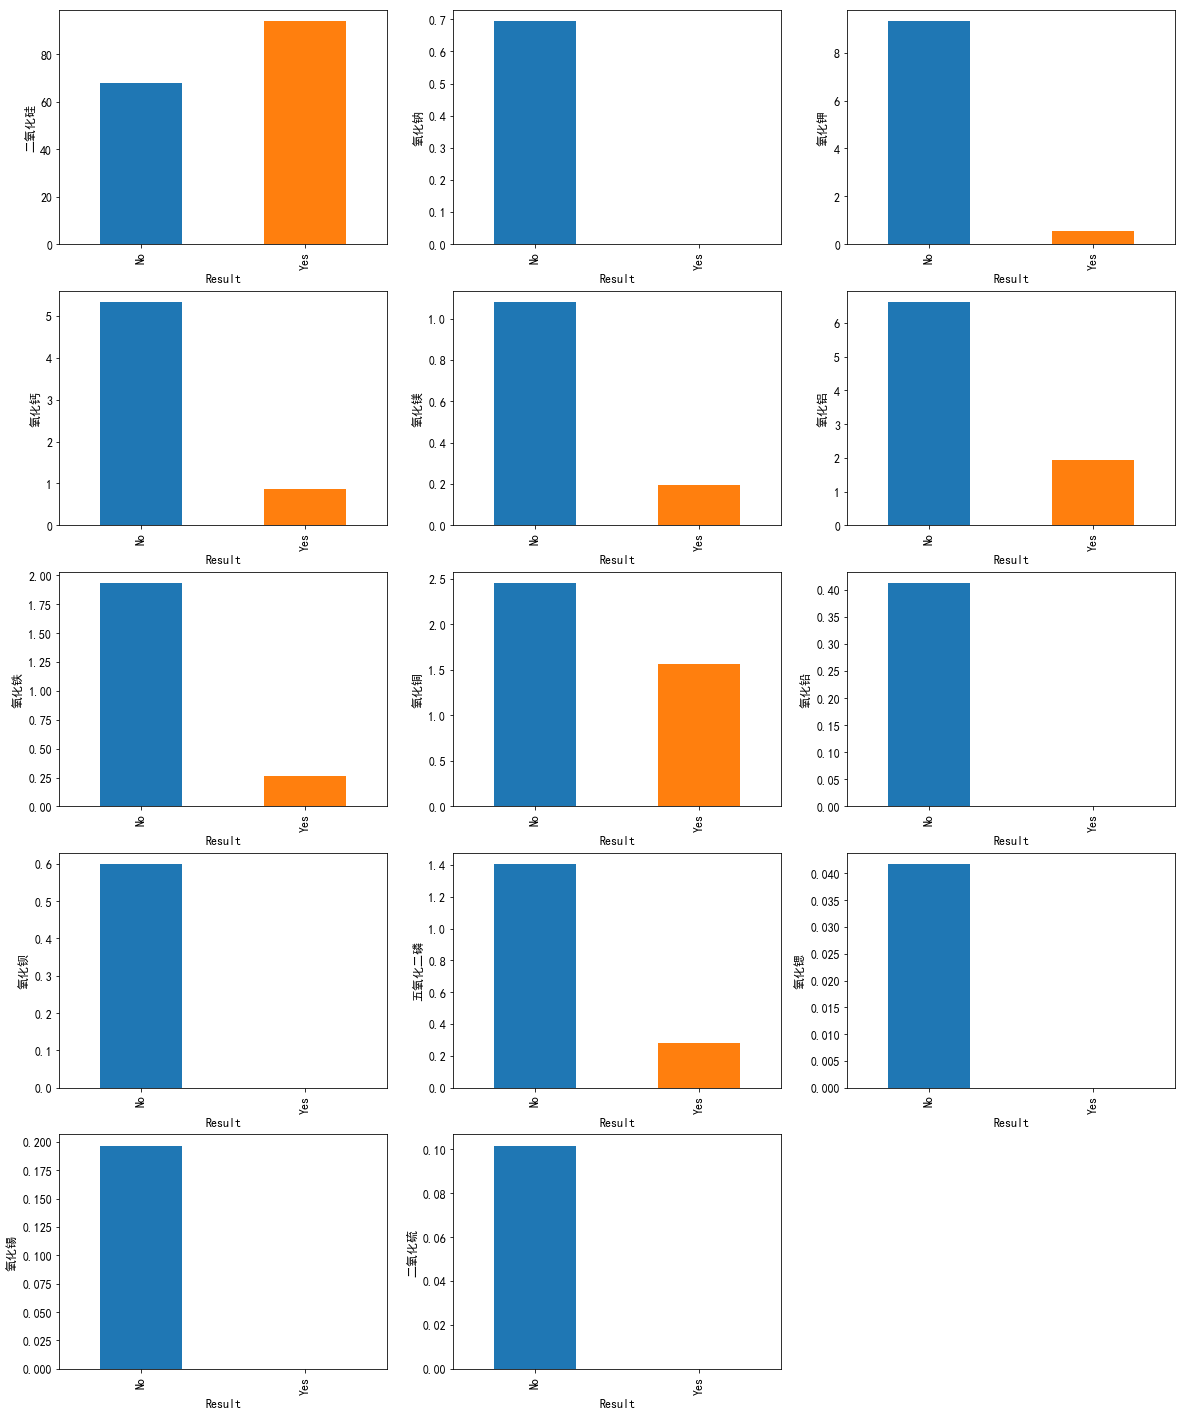
\includegraphics[width=0.7\textwidth]{8.png} %插入图片,[]中设置图片大小,{}中是图片文件名
	\caption{高钾类玻璃风化与各化学成分关系直方图} %最终文档中希望显示的图片标题
	\label{Fig.main9} %用于文内引用的标签
\end{figure}


由图8可知高钾玻璃中含氧化钠、氧化铅、氧化钡、氧化锶、氧化锡以及二氧化硫等化学分成表面未风化的均值较高,而表面风化的均值为0;氧化钾、氧化钙、氧化镁、氧化铝、氧化铁、五氧化二磷等化学分成表面未风化的均值均远大于表面风化的均值;由此可知风化的玻璃中含有氧化钠、氧化铅、氧化钡、氧化锶、氧化锡以及二氧化硫等化学成分含量较少,而含氧化钾、氧化钙、氧化镁、氧化铝、氧化铁、五氧化二磷等成分相对于多一些;另外,由于二氧化硅为玻璃制作的主要原材料,在化学成分中分布很广,在分析与玻璃风化是否有联系的结果并不是很明显。故玻璃风化联系最紧密的化学成分是氧化铜,所有化学成分与玻璃未风化联系都紧密。

同理本文可得到铅钡类玻璃风化与各化学成分关系的直方图如下:


\begin{figure}[H] 
	\centering %图片居中
	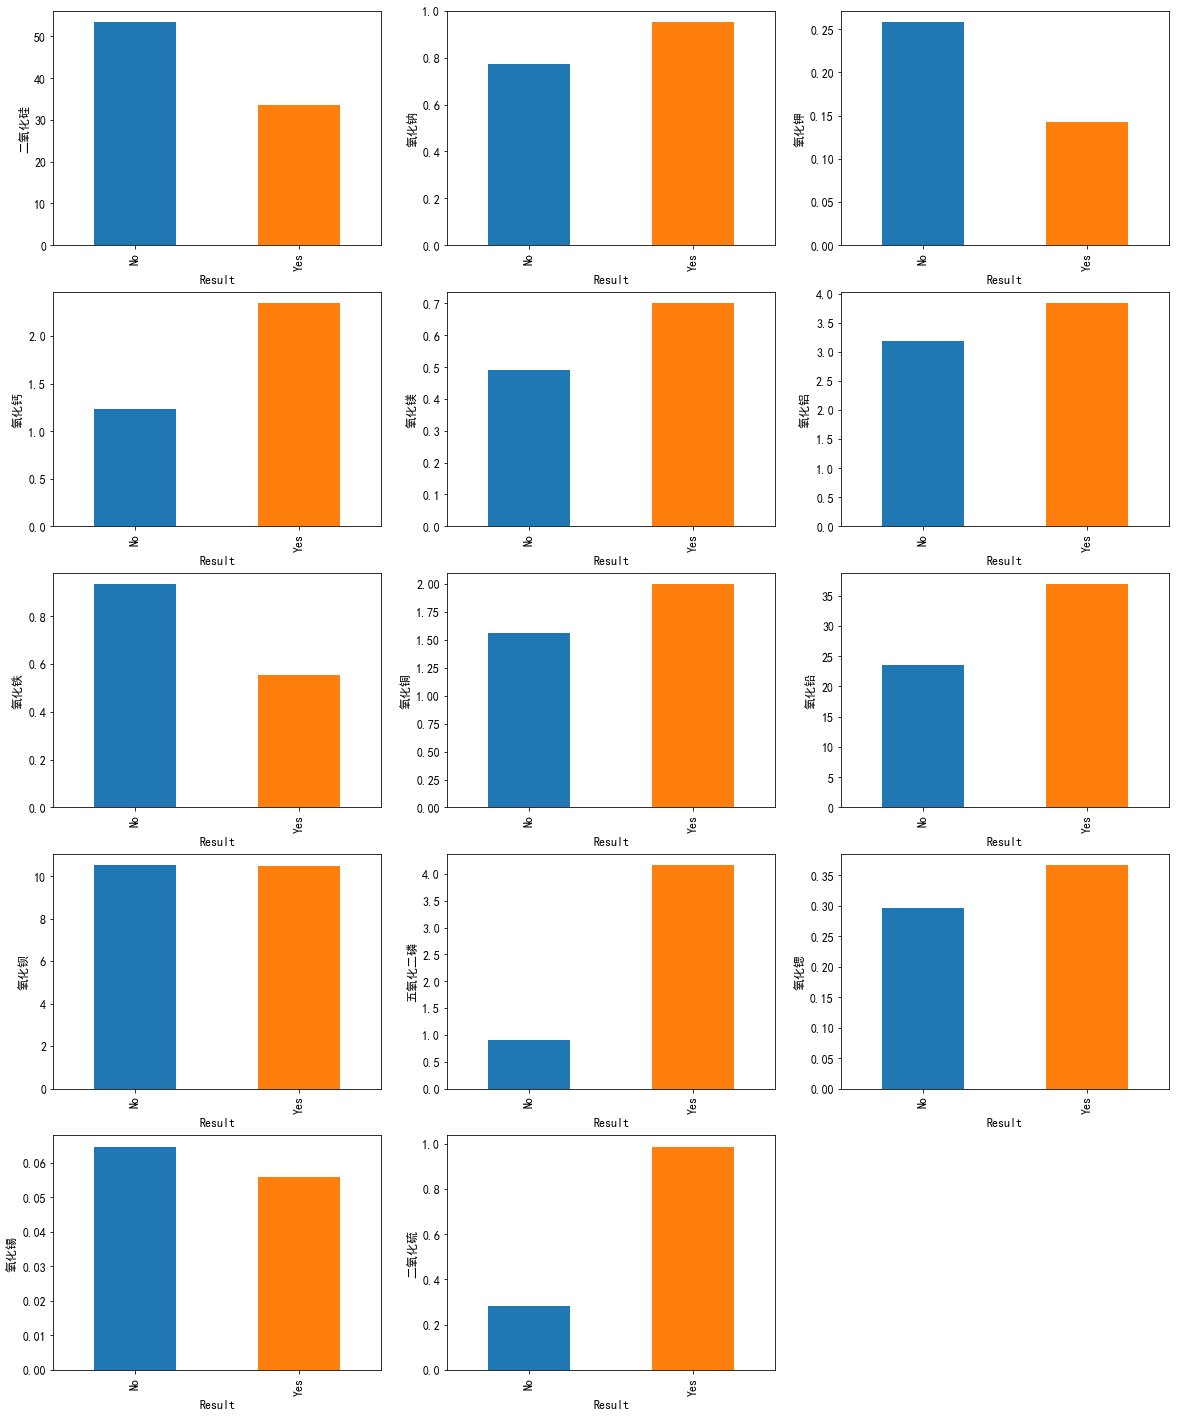
\includegraphics[width=0.7\textwidth]{9.png} %插入图片,[]中设置图片大小,{}中是图片文件名
	\caption{铅钡类玻璃风化与各化学成分关系直方图} %最终文档中希望显示的图片标题
	\label{Fig.main10} %用于文内引用的标签
\end{figure}

由图9知对于铅钡类玻璃中二氧化硫与五氧化二磷两种化学成分表面风化均值占比远高于表面未风化均值;而二氧化硅、氧化钾、氧化镁三个化学成分中玻璃表面风化均值低于表面未风化的均值;其余化学成分与表面是否风化占比相差不大。故二氧化硫与五氧化二磷两种化学成分绝大多数被风化,其余化学成分风化与被风化的程度相差不大。

\subsubsection{显著性检验考察风化情况下各化学成分差异性}

依据以上得到的数据可视化图,为了检验风化前后化学成分是否有明显变化,分别对高钾玻璃和铅钡玻璃风化前后对应的化学成分进行显著性检验。首先进行正态性检验得到下表:

\begin{table}[H]
	\centering
	\begin{tabular}{c c c c c c c} 
	    \toprule[1.5pt]    
		二氧化硅 & 氧化钠 & 氧化钾 & 	… & 氧化锶 & 氧化锡 & 二氧化硫 \\
		\midrule[1pt]
		0 &	0.002680 &	0 &	… &	0.002680 &	0.002680 &	0.002680 \\
	    \toprule[1.5pt]
	\end{tabular}
\caption{高钾玻璃化学成分正态检验部分表}
\end{table}

由上表发现化学成分均未通过正态性检验。

假设风化前后的化学成分有显著性差异,对于通过正态性检验的成分进行配对样本t检验,结果如下:

\[p\_value = 0.10991037\]

故拒绝原假设,氧化铜在高钾玻璃风化前后不具有显著差异。

假设风化前后的化学成分有显著性差异,对于未通过正态性检验的成分进行配对Milcoxon检验,结果如下:

\begin{table}[H]
	\centering
	\begin{tabular}{c c c c c c c} 
		\toprule[1.5pt]
		二氧化硅 &	氧化钠 & 氧化钾 &	… &	氧化锶 & 氧化锡 &	二氧化硫 \\
		\midrule[1pt]
		0.002526 &	0.181449 &	0.003263 &	… &	0.5 & 1 & 0.181449 \\
		\toprule[1.5pt]
	\end{tabular}
\caption{配对检验表}
\end{table}

氧化钠、氧化铜、氧化钡、氧化锶、二氧化硫五种成分拒绝原假设,在高钾玻璃风化前后不具有显著性差异;其他成分接受原假设,在风化前后具有显著性差异。
同理可得铅钡玻璃化学成分正态性检验表:

\begin{table}[H]
	\centering
	\begin{tabular}{c c c c c c c} 
		\toprule[1.5pt]
		二氧化硅 & 氧化钠 & 氧化钾 & … & 氧化锶 & 氧化锡 & 二氧化硫 \\
		\midrule[1pt]
		0.279 & 0.001*** &	0.005*** &	… &	0.585 &	0.000*** & 0.000*** \\
		\toprule[1.5pt]
	\end{tabular}
\caption{铅钡玻璃化学成分正态检验部分表}
\end{table}

由上表得:化学成分氧化钠、氧化钾、氧化铁、氧化锡、二氧化硫未通过正态性检验,化学成分二氧化硅、氧化钙、氧化镁、氧化铝、氧化铜、氧化铅、氧化钡、五氧化二磷、氧化锶通过正态性检验。

假设风化前后的化学成分有显著性差异,对于未通过正态性检验的成分进行配对Milcoxon检验,结果如下:

\begin{table}[H]
	\centering
	\begin{tabular}{c c c c c c c} 
		\toprule[1.5pt]
		二氧化硅 &	氧化钠 & 氧化钾 &	… &	氧化锶 & 氧化锡 & 二氧化硫 \\
		\midrule[1pt]
		0.000*** & 0.273 & 0.894 & … & 0.217 & 0.001*** & 0.225 \\
		\toprule[1.5pt]
	\end{tabular}
\caption{配对检验表}
\end{table}

二氧化硅、氧化钙、氧化镁、氧化铝、氧化铜、氧化铅、氧化钡、五氧化二磷、氧化锶九种成分拒绝原假设,在铅钡玻璃风化前后不具有显著性差异;其余化学成分不拒绝原假设,其他成分接受原假设,在风化前后具有显著性差异。


\subsection{预测风化前的化学成分含量}

\subsubsection{高钾、铅钡玻璃风化前后数据分析}

把高钾和铅钡玻璃对表面是否风化的数据分别进行分析,得到部分结果如下表详情见附件。

\begin{table}[H]
	\centering
	\begin{tabular}{c c c c c c} 
        \toprule[1.5pt]
		 & 二氧化硅 & 氧化钠 & 氧化钡 & 二氧化硫	& 五氧化二磷 \\
        \midrule[1pt]
		数量 & 12.00000 & 12.00000 & 12.00000 & 12.00000 & 12.00000 \\
		总和 & 67.984167 & 0.695000 & 0.598333 & 0.101667 & 1.402500 \\
		占比 & 8.755099 &	1.286917 & 0.982102 & 0.185513 & 1.433959 \\
		最小值	& 59.0100 & 0.0000 & 0.0000 & 0.0000 & 0.0000 \\
		$\frac{1}{4}$百分点 & 61.6775 & 0.0000 & 0.0000 & 0.0000 &	0.6900 \\
		$\frac{1}{2}$百分点 & 65.5300 & 0.0000 & 0.0000 & 0.0000 & 1.0200 \\
		$\frac{3}{4}$百分点 &  71.1675 & 0.5250 & 1.0725 &	0.0000 &	1.2925 \\
		最大值 & 87.050000 & 3.380000 & 2.860000 & 2.360000 & 4.500000 \\
		\toprule[1.5pt]
	\end{tabular}
\caption{高钾类玻璃风化前部分数据分析}
\end{table}

接下来对高钾玻璃风化前后数据进行可视化,得到以下可视化分布图:

\begin{figure}[H] 
	\centering %图片居中
	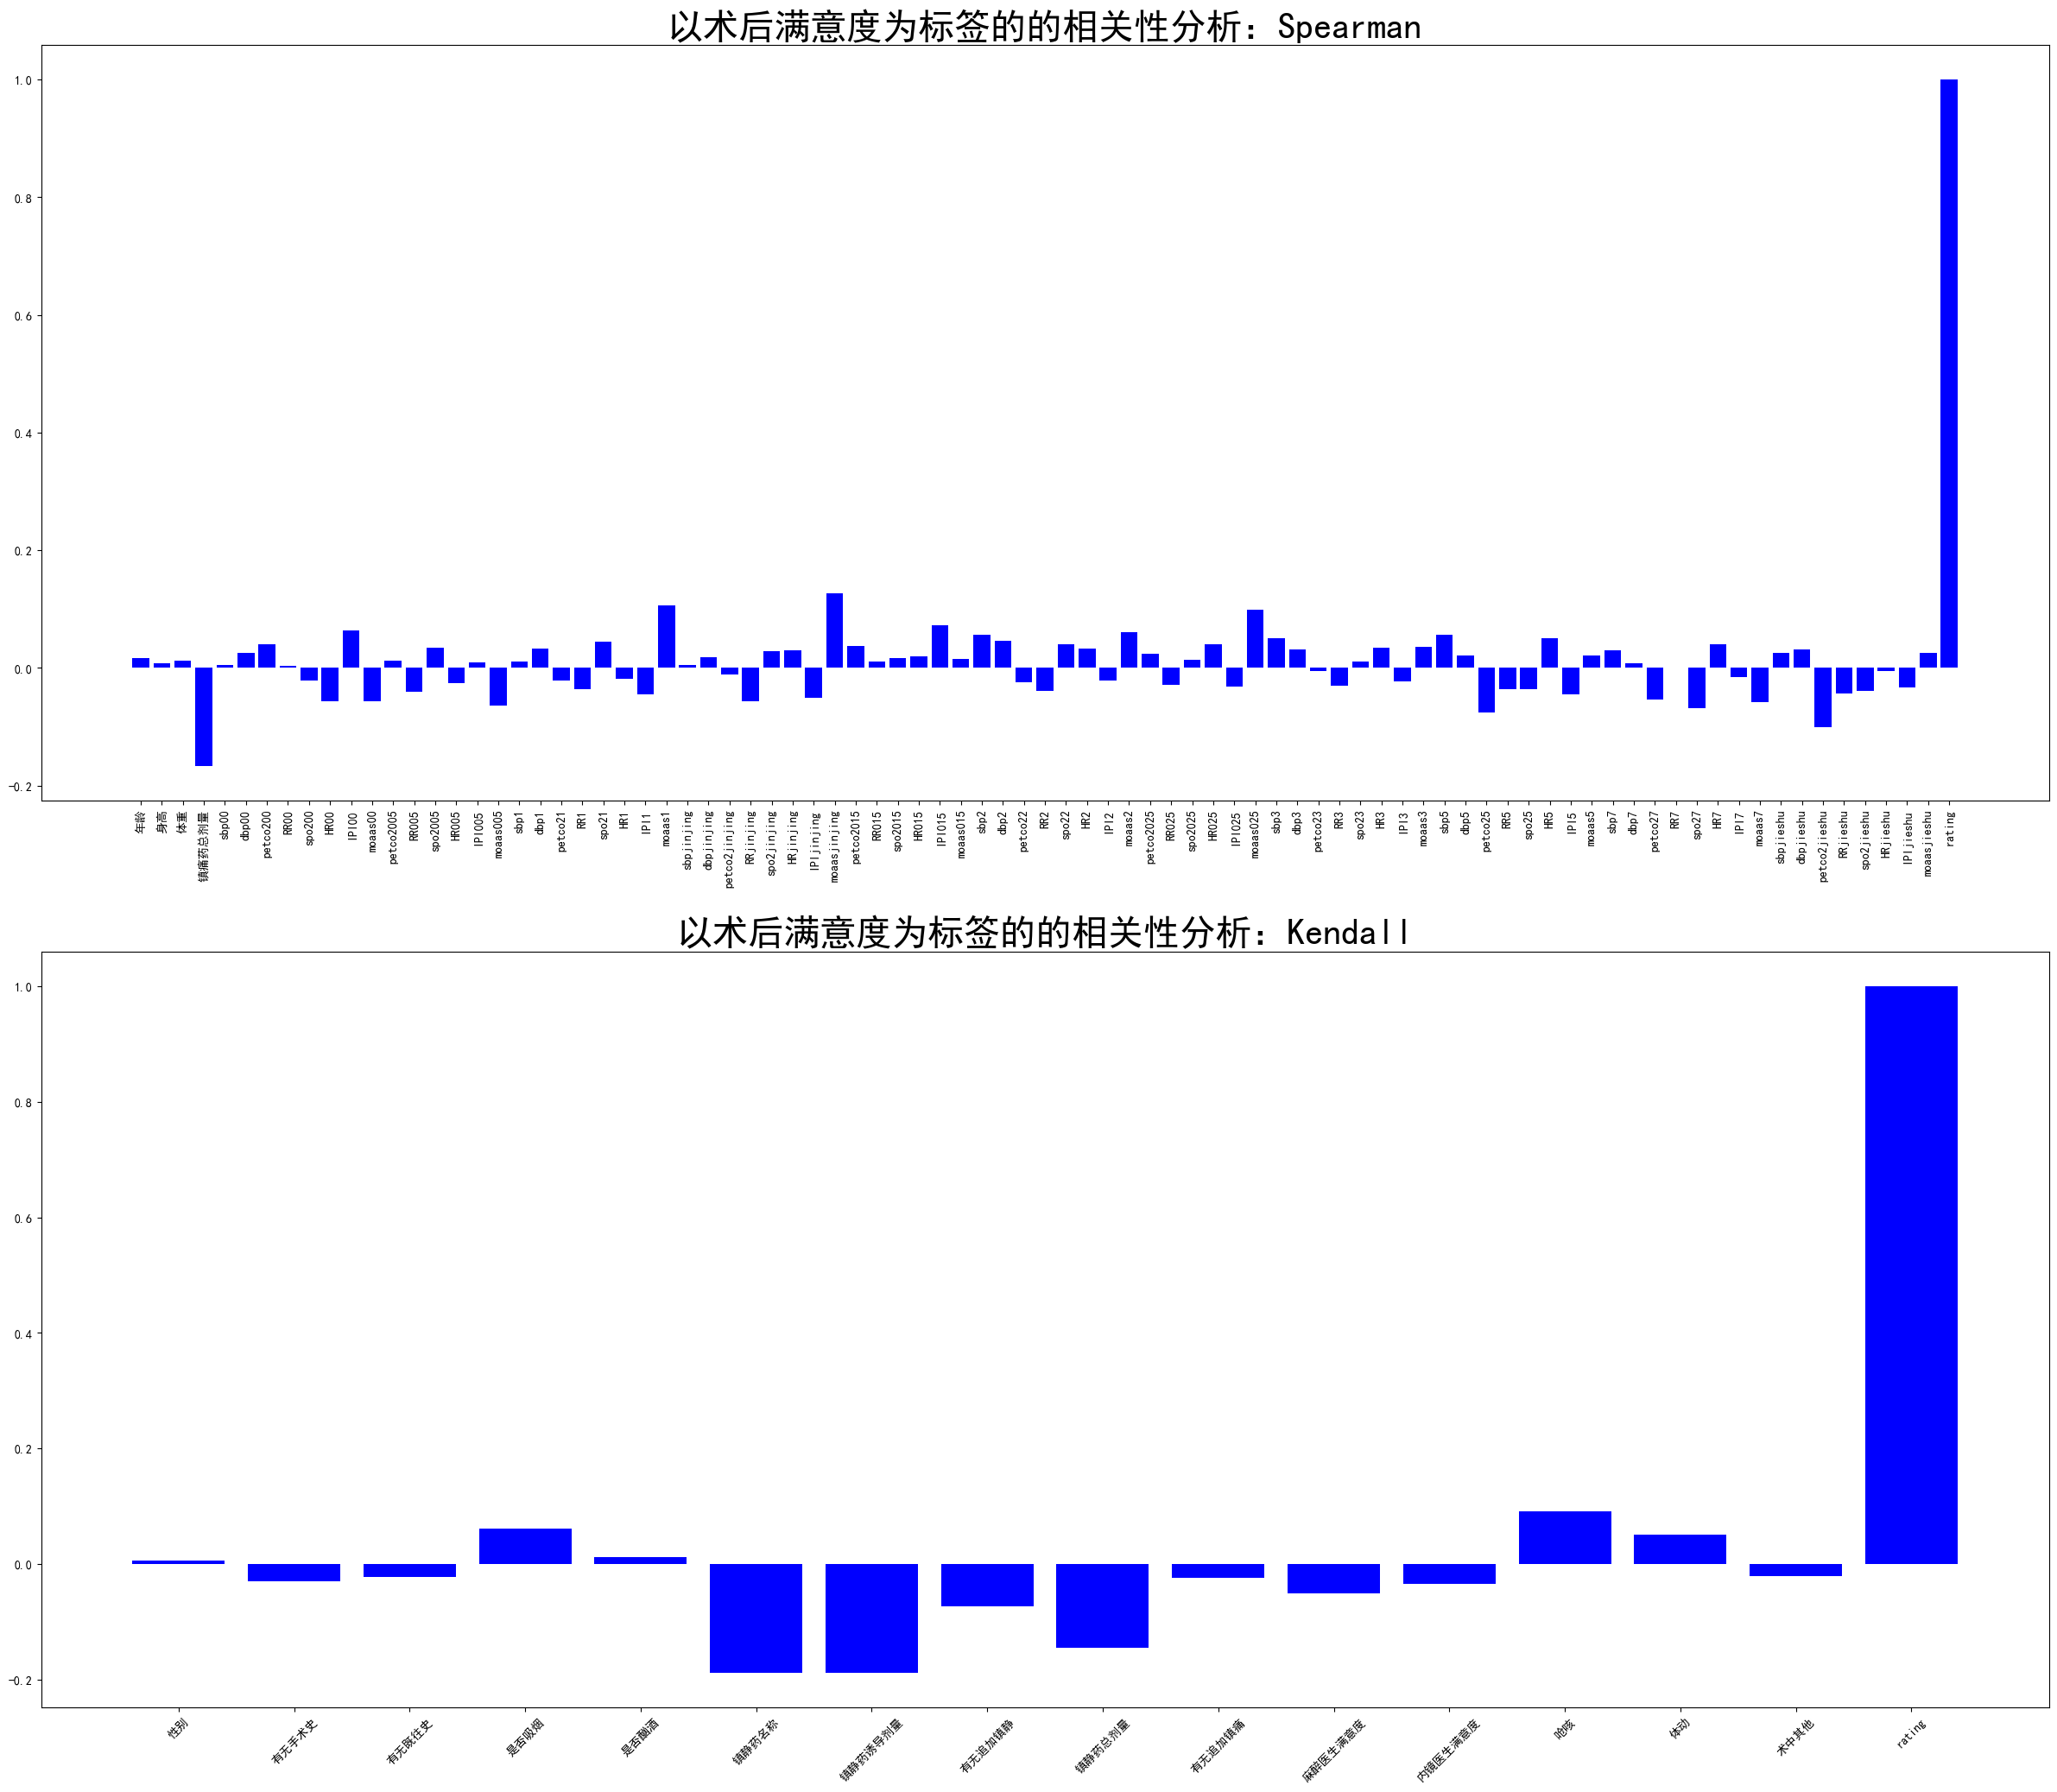
\includegraphics[width=0.7\textwidth]{10.png} %插入图片,[]中设置图片大小,{}中是图片文件名
	\caption{左图为高钾玻璃风化前各成分分布图;右图为高钾玻璃风化后各成分分布图} %最终文档中希望显示的图片标题
	\label{Fig.main11} %用于文内引用的标签
\end{figure}

调用Matplotlib的boxplot函数对高钾玻璃风化前后各特征的分布进行可视化,查看各特征离群值数量的多少。通过图10可以见高价玻璃风化前后各个化学成分的离群值较少,因此通过平均数可以反应数据各特征的一般水平。

\begin{figure}[H] 
	\centering %图片居中
	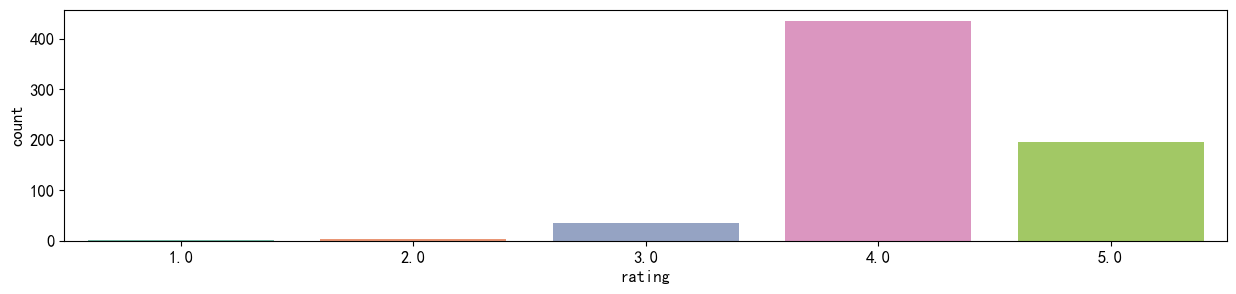
\includegraphics[width=0.7\textwidth]{11.png} %插入图片,[]中设置图片大小,{}中是图片文件名
	\caption{左图为铅钡玻璃风化前各成分分布图;右图为铅钡玻璃风化后各成分分布图} %最终文档中希望显示的图片标题
	\label{Fig.main12} %用于文内引用的标签
\end{figure}

通过图11可得铅钡玻璃风化前后各个化学成分的离群值依然较少,因此可以通过平均数来反映数据各个特征的一般水平。

\subsubsection{求取平均值、预测风化前化学成分}

由上把高钾和铅钡玻璃数据分析后可得数据异常值较少,为寻找一个风化前后具有代表性的数据,本问对两种玻璃风化前后的数据分别求平均值,具体方法如下:

1. 根据公式

\begin{equation}
    \overline{{{y}_{ijz}}}=\frac{\sum{{{y}_{ijz}}}}{{{n}_{ijz}}}.
\end{equation}

可分别求出高钾玻璃和铅钡玻璃风化前后每种化学成分的平均值。

2. 对风化后数据异常值进行检验,发现没有异常值,根据得到的风化前后的数据平均值求出对应化学成分的平均含量比率作为该化学含量的一般比率。设$H_j$为第$j$类化学物质的比例系数,利用公式

\begin{equation}
    {{H}_{ij}}=\frac{\overline{{{y}_{iy1}}}}{\overline{{{y}_{iy2}}}}.
\end{equation}

分别得到高钾和铅钡玻璃风化前后各成分比例系数部份表如下,具体详情见附件:


\begin{table}[H]
	\centering
	\begin{tabular}{c c c} 
		\toprule[1.5pt]
		成分类型 & 高钾玻璃风化前后含量比值 & 铅钡玻璃风化前后含量比值 \\
		\midrule[1pt]
		二氧化硅 & 0.723518 & 2.145246 \\
		五氧化二磷 & 5.008929 & 0.171270 \\
		氧化钾 & 6.129310 & 1.936599 \\
		氧化钙 & 5.487288 & 0.456906 \\
		氧化镁	& 3.430052 & 0.757396 \\
		氧化铝	& 7.289308 & 7 1.075628 \\
		\toprule[1.5pt]
	\end{tabular}
\caption{风化前后比例系数表}
\end{table}



最后再通过公式

\begin{equation}
    y_{iy1}^{'}={{H}_{ij}}\cdot y_{iy2}^{'}.
\end{equation}

求出风化后的玻璃对应的风化前的化学物质含量,得到对应的部分结果如下表所示,详情见附件:

\begin{table}[H]
	\centering
    \begin{tabular}{c c c c c c} 
        \toprule[1.5pt]
        样本检测位点成分 &	二氧化硅 &	氧化钠 & 	\dots &	氧化锡 &	二氧化硫 \\
        \midrule[1pt]
        01 &	77.82951415 &	0 &	\dots &	0 &	0 \\
        02 &	67.01947595 &	0.695 &	\dots &	0.196666667 &	0.101666667 \\
        03 &	43.20524848 &	0 &	\dots &	0 &	0.531689189 \\
        \dots &	\dots &	\dots &	\dots &	\dots &	\dots \\
        31 &	54.5321458 &	0 &	\dots &	0 &	0 \\
        32 &	65.19401695 &	0 &	\dots &	0 &	0 \\
        \toprule[1.5pt]
    \end{tabular}
    \caption{风化前化学成分含量部分}
\end{table} 



% ------------------------------------------------------------ %
%    打开chapter文件夹里的问题二建模.tex文件,编辑其中的内容
% ------------------------------------------------------------ %
%    打开chapter文件夹里的问题二建模.tex文件,编辑其中的内容
% ------------------------------------------------------------ %
\section{问题二建模与求解}

为分析高钾和铅钡两类玻璃的分类规律;对于每个类别选择合适的化学成分对其进行亚类划分得出分类结果,并对分类结果的合理性和敏感性进行分析,做流程图如下: 

\begin{figure}[H] 
	\centering %图片居中
	\includegraphics[width=0.7\textwidth]{12.png} %插入图片,[]中设置图片大小,{}中是图片文件名
	\caption{问题二流程图} %最终文档中希望显示的图片标题
	\label{Fig.main13} %用于文内引用的标签
\end{figure}

\subsection{模型准备}

\subsubsection{数据预处理}

用Pandas读取数据后用isnull函数查找缺失值,发现表中数据有缺失值,用众数来补全数据中的缺失值,再次检验未见异常值。

\subsubsection{特征工程}

要求分别在高钾玻璃和铅钡玻璃的化学成分中选择合适的特征进行亚类分析,聚类分析由于以欧几里得距离为组间、组内判别的衡量,往往对特征的要求极高。
先对原来的14个化学成分指标进行标准化:
再利用方差筛选法来对这几个特征进行过滤筛选,公式为:

\begin{equation}
    \sigma_{j}^{2}=\frac{\sum{{{({{y}_{j}}-\overline{{{y}_{j}}})}^{2}}}}{{{n}_{j}}},j=1,\cdots ,14
\end{equation}

求出第$j$类化学成分的的方差值。为了筛选到最优方差范围,取不同方差值检验化学成分数据通过情况,得到方差通过如下表:

\begin{table}[H]
	\centering
	\begin{tabular}{c c c c c} 
		\toprule[1.5pt]
		方差 & 二氧化硅 & 氧化钠 & \dots & 二氧化硫 \\
		\midrule[1pt]
		$\sigma^2=0$ & 未通过 & 未通过 & \dots & 未通过 \\
		\dots & \dots & \dots & \dots & \dots \\
		$\sigma^2=5$ & 通过 & 未通过 & dots & 未通过 \\
		\dots & \dots & \dots & \dots & \dots \\
		$\sigma^2=10$ & 通过 & 未通过 & \dots & 未通过 \\
		\toprule[1.5pt]
	\end{tabular}
\caption{方差通过情况表}
\end{table}

方差等于10已经能够较充分的分离特征明显的变量,故令数据
\begin{equation}
    {\sigma_j}^2 \leq 10
\end{equation}

利用方差法筛选选出特征明显的变量,用VarianceThreshold函数分别选出高钾类玻璃和铅钡类玻璃化学成分主要特征值,结果如下:

\begin{table}[H]
	\centering
	\begin{tabular}{c c c c c} 
		\toprule[1.5pt]
		高钾类玻璃 & 二氧化硅 & 氧化钾 & 氧化钙 & 氧化铝 \\
		\midrule[1pt]
		铅钡类玻璃 & 二氧化硅 & 氧化钡 & 氧化铅 & 五氧化二磷 \\
		\toprule[1.5pt]
	\end{tabular}
\caption{方差筛选后特征}
\end{table}


\subsection{数据可视化浅析高钾玻璃和铅钡玻璃分类规律}

根据以上得到的数据,本文把14个化学成分作为数值特征与玻璃类型(高钾玻璃和铅钡玻璃)进行多变量数据可视化分析,利用matplotlib库得到数据可视化图如下:

\begin{figure}[H] 
	\centering %图片居中
	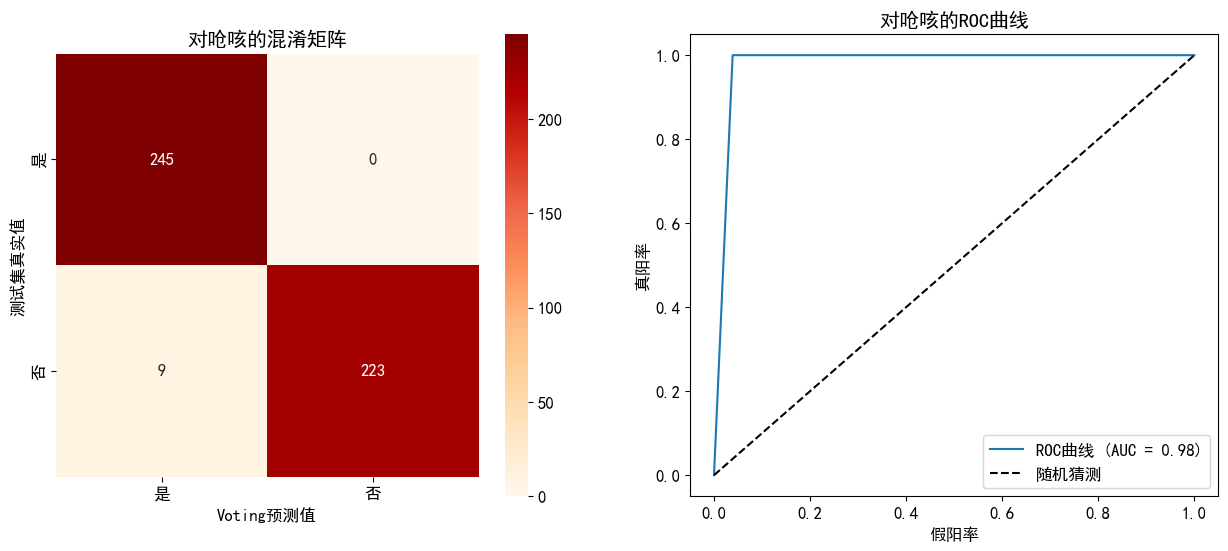
\includegraphics[width=0.7\textwidth]{13.png} %插入图片,[]中设置图片大小,{}中是图片文件名
	\caption{数据可视化图} %最终文档中希望显示的图片标题
	\label{Fig.main14} %用于文内引用的标签
\end{figure}

由图13可知氧化铅、氧化钡、氧化锶、二氧化硫、氧化钾五种化学成分在两种玻璃类型中占比相差极大,其中氧化铅、氧化钡、氧化锶、二氧化硫四种化学成分在高钾类玻璃的含量占比远大于铅钡类玻璃;而氧化钾在高钾类玻璃的含量占比远小于于铅钡类玻璃;氧化钙、氧化锡、氧化铁三种化学成分在高钾类玻璃的含量占比略大于铅钡类玻璃;氧化钠和五氧化二磷两种化学成分在高钾类玻璃的含量占比略于于铅钡类玻璃;而氧化镁、氧化铜两种化学成分在两类玻璃的占比相差不大。

接下来本文分析两个分类特征——纹饰和颜色与玻璃类型之间的关系,分别作多变量分析可视化进行分析,得到数据可视化图如下:

\begin{figure}[H] 
	\centering %图片居中
	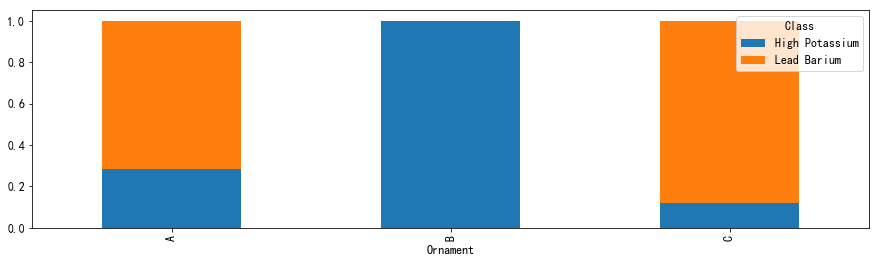
\includegraphics[width=0.7\textwidth]{14.png} %插入图片,[]中设置图片大小,{}中是图片文件名
	\caption{纹饰与玻璃类型可视化图} %最终文档中希望显示的图片标题
	\label{Fig.main15} %用于文内引用的标签
\end{figure}

图14可看出A类纹饰中高钾类玻璃占百分之七十左右,占比大于铅钡类玻璃占比,B类纹饰全是高钾类玻璃,而C类纹饰中高钾类约占百分之九十以上,远大于铅钡类玻璃占比。

\begin{figure}[H] 
	\centering %图片居中
	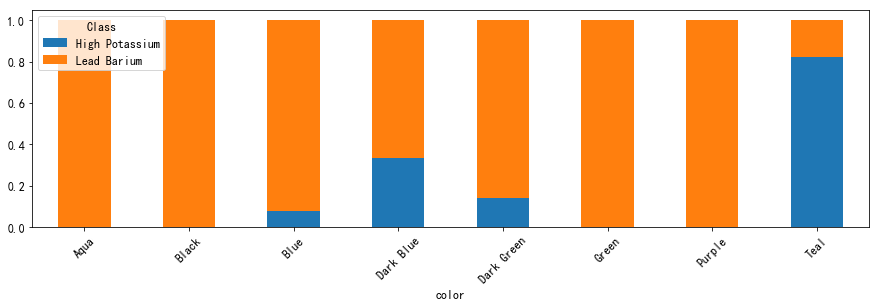
\includegraphics[width=0.7\textwidth]{15.png} %插入图片,[]中设置图片大小,{}中是图片文件名
	\caption{纹饰与玻璃类型可视化图} %最终文档中希望显示的图片标题
	\label{Fig.main16} %用于文内引用的标签
\end{figure}

图15可知浅蓝色样本玻璃中高钾类玻璃占比较大,蓝色、深蓝、深绿三种颜色玻璃中高钾类玻璃占比较小,而其余颜色玻璃中全为铅钡类玻璃。

综上所述,B类纹饰以及蓝绿色、黑色、绿色、紫色的玻璃全为高钾类玻璃;浅蓝色玻璃大部分为高钾玻璃,C类纹饰与蓝色、深绿色玻璃绝大多数多铅钡玻璃。可以得到如下显性分类结果表:

\begin{table}[H]
	\centering
	\begin{tabular}{c c} 
		\toprule[1.5pt]
		高钾玻璃 & B类纹饰、蓝绿色、黑色、绿色、紫色 \\
		\midrule[1pt]
		铅钡玻璃 & C类纹饰、蓝色、深绿色 \\
		\toprule[1.5pt]
	\end{tabular}
\caption{显性分类规律表}
\end{table}

上表可以直观得到两种玻璃的分类标准,下面为了更进一步的分析它们内部分类的本质性规律,决定采用决策树得到内部规律分类。

\subsection{巧用决策树二叉树结构分析两类玻璃分类依据}

决策树是一种经典的传统机器学习分类器,因其独特的树状分类机制,可以让操作者在建模完成后通过调用plot\_tree函数了解每一次树枝分叉的条件,这一特点可以直接达成对玻璃分类依据的探究。

\subsubsection{计算决策树分类结果与本身标签吻合度}

附件早已给出各个样本的玻璃类别,本文通过决策树分类器寻找分类标准,一大前提就是当前决策树的分类结果和玻璃自身标签完全吻合,本文通过混淆矩阵计算决策树分类结果与样本本身标签的吻合度,结果如下:

\begin{figure}[H] 
	\centering %图片居中
	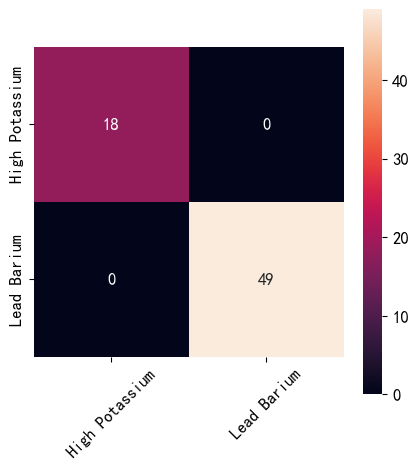
\includegraphics[width=0.7\textwidth]{16.png} %插入图片,[]中设置图片大小,{}中是图片文件名
	\caption{决策树预测结果与样本标签混淆矩阵} %最终文档中希望显示的图片标题
	\label{Fig.main17} %用于文内引用的标签
\end{figure}

由混淆矩阵热力图可知,使用决策树预测的结果与样本自身标签完全匹配。

\subsubsection{决策树的树状结构导出}

通过决策树独特的属性,从sklearn.tree中导入函数plot\_tree作出决策树模型的树状结构,图形如下:

\begin{figure}[H] 
	\centering %图片居中
	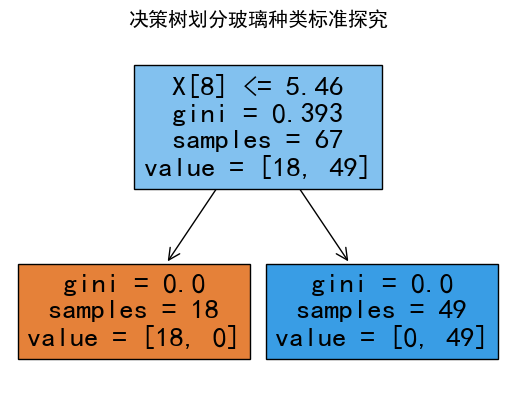
\includegraphics[width=0.7\textwidth]{17.png} %插入图片,[]中设置图片大小,{}中是图片文件名
	\caption{决策树树状结构可视化} %最终文档中希望显示的图片标题
	\label{Fig.main18} %用于文内引用的标签
\end{figure}

通过此图形,本文惊人地发现:决策树所挖掘的数据内在的分类标准与之前看似合理、充分的结果相差甚远——玻璃类比的划分居然只与氧化铅的含量有关!这也进一步告诉本文,简单的数据可视化分析往往只能摸索出浅层次的结论,想要挖掘数据深层次的联系必须通过合适的数据与算法。

\subsection{聚类分析—层次聚类法}

为了对化学成分进行更深层次的分析,又由表8可知每类玻璃分别选出4个变量进行类别划分,利用python中的层次聚类法函数选取三类指标进行划分,分类结果如下表:

\begin{table}[H]
	\centering
	\begin{tabular}{c c c c} 
		\toprule[1.5pt]
		& 第一类 & 第二类 & 第三类 \\
		\midrule[1pt]
		样本编号 & 03,10,12,13,14,18,21,22,27 & 07,09 & 01,04,05,06,15,16,17 \\
		\toprule[1.5pt]
	\end{tabular}
\caption{显性分类规律表}
\end{table}


\begin{table}[H]
	\centering
	\begin{tabular}{c c c c} 
		\toprule[1.5pt]
		& 第一类 & 第二类 & 第三类 \\
		\midrule[1pt]
		样本编号 & 02,19,20,23,32,33,37,39,41,42,43,44,47,48,54,55,56,57,58 & 24,26,30,31,34,35,36,38,40,45,46,49,50,51,52,53	& 08,11,25,28,29 \\ 
		\toprule[1.5pt]
	\end{tabular}
\caption{铅钡类划分结果表}
\end{table}

下面对分类合理性进行检验。

\subsubsection{合理性检验}

本文的目的是为了对分类结果的合理性和敏感性,在对聚类分析结果进行检验时,仅用轮廓系数判断是有失可信度的,CH分数、戴维森堡丁指数(DBI)是对聚类效果评估好坏的评价另外两种方式,下面利用python使用以上三种方法对结果进行检验,得到如下结果:


\begin{table}[H]
	\centering
	\begin{tabular}{c c c c} 
        \toprule[1.5pt]
	    & 轮廓系数 & CH分数 & DBI \\
	    \toprule[1.5pt]
	    高钾玻璃 & 0.448406754 & 36.65655497 & 0.87395307 \\
	    \midrule[1pt]
	    铅钡玻璃 & 0.446694394 & 45.85302210 & 0.82682893 \\
	    \toprule[1.5pt]
	\end{tabular}
\caption{检验结果表}
\end{table}


由上表可知,两类玻璃所得的轮廓系数接近0.5,说明同类样本相距比较接近,聚类效果比较好;CH分数是通过评估类之间方差和类内方差来计算得分,分值越大,表示聚类效果越好,DDB值越小表示聚类结果同簇内部紧密,不同簇分离较远。即类内距离越小,类间距离越大,综上可得出聚类效果较好,该划分方法合理。



\subsubsection{扰动处理}

敏感性分析有很多方法可以实现,依题意所言对结果进行敏感性分析,即探究模型的鲁棒性。本文对被预测标签的数据集进行一定程度的扰动处理,再次预测后通过比较干扰前后的标签差异来衡量模型的稳定性。另外,本文不断对各个特征分别加大干扰,以求探究出影响模型划分类别的“阈值”,用表示高钾玻璃的扰动值,其中表示铅钡玻璃的扰动值,利用公式:

\begin{equation}
    error{{1}_{j}}=\overline{{{y}_{j1}}}*d,d\in \left( 0,+\infty  \right)
\end{equation}

\begin{equation}
    error{{2}_{j}}=\overline{{{y}_{j2}}}*d,d\in \left( 0,+\infty  \right)
\end{equation}

得到每种化学成分的扰动值,带到模型中进行扰动检验,可以得到敏感阈值,最后得出两类玻璃亚类分化的噪音百分比图:

\begin{figure}[H] 
	\centering %图片居中
	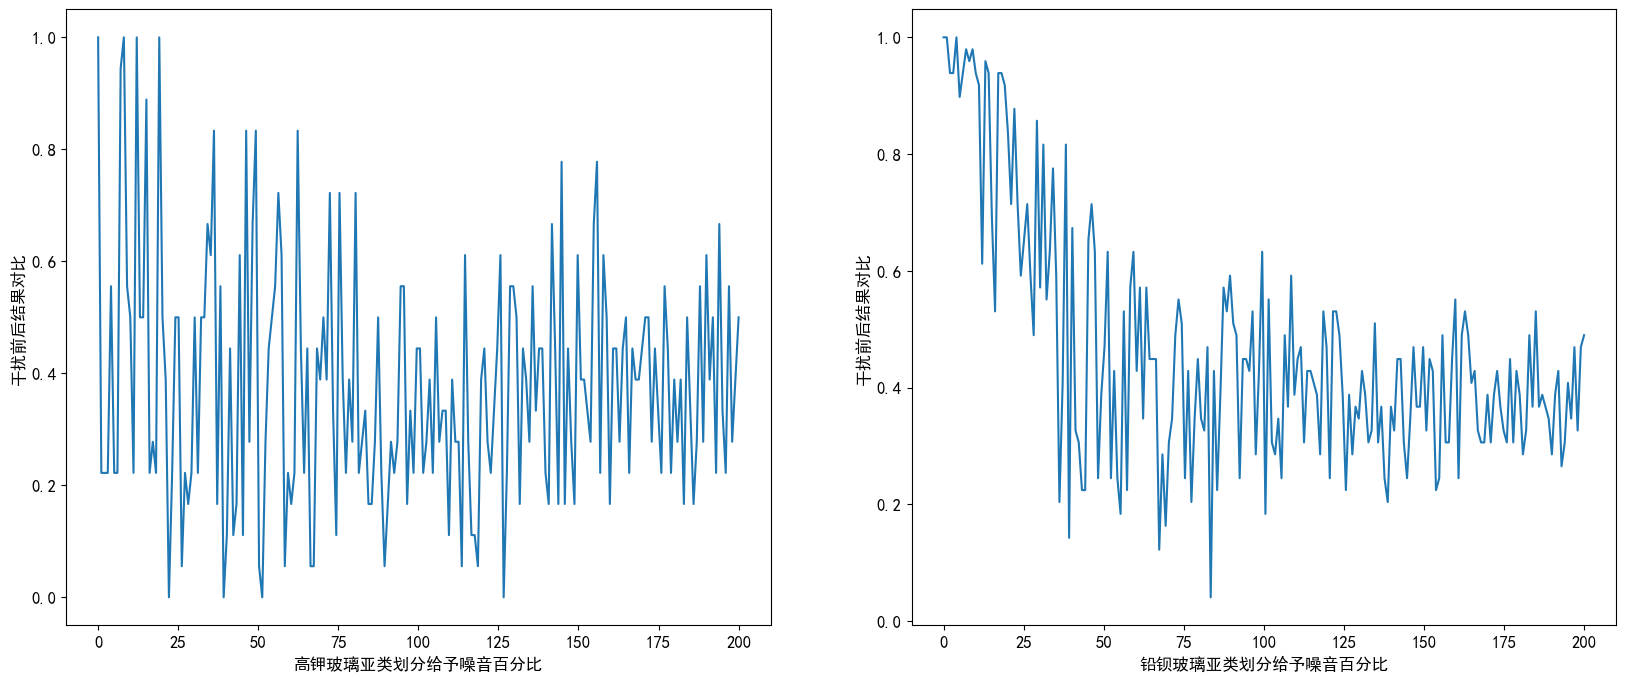
\includegraphics[width=0.7\textwidth]{18.png} %插入图片,[]中设置图片大小,{}中是图片文件名
	\caption{左图为高钾玻璃亚类分化噪音百分比图;右图为铅钡玻璃亚类分化噪音百分比图} %最终文档中希望显示的图片标题
	\label{Fig.main19} %用于文内引用的标签
\end{figure}

通过图18(左)可看出该模型的敏感性阈值d在(0,0.25)之间,模型的准确率都在20\%以上,当d大于0.25时模型的准确率波动性大,预测准确率变化大,因此最好将数据敏感性阈值控制在0.25以内。而对于右图可发现模型的敏感性阈值d在(0,0.1)之间模型的准确率都在90\%以上,当d大于0.10时模型的准确率波动性大,准确率变化大,最好将数据敏感性阈值控制在0.10以内。



% ------------------------------------------------------------ %
%    打开chapter文件夹里的问题三建模.tex文件,编辑其中的内容
% ------------------------------------------------------------ %
%    打开chapter文件夹里的问题三建模.tex文件,编辑其中的内容
% ------------------------------------------------------------ %
\section{问题三建模与求解}

\subsection{数据预处理}

通过Pandas库进行数据读取,使用isnull函数查找数据中的缺失值,对于附件表单3中缺失值进行补0,并对于表中样本化学成分含量求和,均满足85\%—105\%,无需对数据进行删减。

\subsection{未知类别文物预测模型}

\subsubsection{模型准备}

模型选择前文从附件表二处理后(补齐缺失值,删除不满足条件只值)的数据中提取的14个化学成分和风化情况这15个特征。以原数据为标准,将数据进行标准化将数据处理到0到1之间。对风化情况进行独热编码。

\subsubsection{模型建立}

投票(voting)在集成学习的分类算法中被广泛运用,投票主要运用软投票(soft voting)是一种对于各基分类器效果融合的模型。本文所选择的4个基分类器分别为线性判别分析、决策树、朴素贝叶斯以及支持向量机。并用voting进行基分类器融合得到一个强分类器。

\begin{figure}[H] 
	\centering %图片居中
	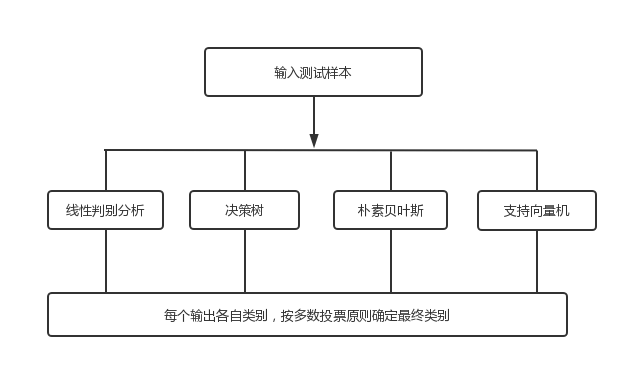
\includegraphics[width=0.7\textwidth]{19.png} %插入图片,[]中设置图片大小,{}中是图片文件名
	\caption{Voting原理} %最终文档中希望显示的图片标题
	\label{Fig.main20} %用于文内引用的标签
\end{figure}



\subsubsection{模型求解}

建立线性判别分析、决策树、朴素贝叶斯以及支持向量机四个性能优良的传统机器学习分类模型,并将训练集分别投入四个模型进行模型训练,通过比较交叉验证后的得分结果,发现四个模型性能均远超过随机分类(成功率0.5)。


\begin{table}[H]
	\centering
	\begin{tabular}{c c} 
		\toprule[1.5pt]
		分类器 & 综合准确率 \\
		\midrule[1pt]
		线性判别分析 & 0.971429 \\
		决策树 & 0.995382 \\
		朴素贝叶斯 & 0.985714 \\
		支持向量机 & 0.985714 \\
		\toprule[1.5pt]
	\end{tabular}
\caption{基分类器评分}
\end{table}

从上表可以看出四种基分类器效果都不错,对于测试集的数据训练准确率都在百分之九十七以上,都是比较好的分类预测模型。

然而四个分类器的分类效果各不相同,所以本着训练性能最优良分类器的原则,本文使用基于结果进行模型融合的VotingClassifier投票算法对四个模型进行融合,公式为:


\begin{equation}
    {{W}_{i}}=\frac{accurac{{y}_{i}}}{\sum\limits_{i=1}^{5}{accurac{{y}_{i}}}}
\end{equation}

软投票的分类结果如下表:

\begin{table}[H]
	\centering
	\begin{tabular}{c c} 
		\toprule[1.5pt]
		分类器 & 综合准确率 \\
		\midrule[1pt]
		VotingClassifier & 1 \\
		\toprule[1.5pt]
	\end{tabular}
\caption{分类结果表}
\end{table}

最后得到了分类预测成功率为1的“完美模型”。
下面对于该分类模型进行评价,利用混淆矩阵热力图如下:


\begin{figure}[H] 
	\centering %图片居中
	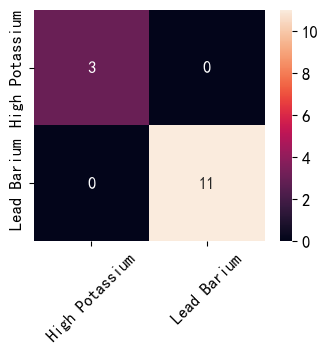
\includegraphics[width=0.7\textwidth]{20.png} %插入图片,[]中设置图片大小,{}中是图片文件名
	\caption{VotingClassifier混淆矩阵热力图} %最终文档中希望显示的图片标题
	\label{Fig.main21} %用于文内引用的标签
\end{figure}


可以看出VotingClassifier分类模型非常完美,是一个非常好的分类器。再基于混淆矩阵的方法对该分类模型进行评价,结合对测试集的预测结果和测试集自身标签、通过计算得到模型的精确度得到如下指标:

\begin{table}[H]
	\centering
	\begin{tabular}{c c c c c} 
		\toprule[1.5pt]
		 & 精确度 & 召回率 & F1分数 & 支持率 \\
        \midrule[1pt]
		铅钡 & 1 & 1 & 1 & 1 \\
		\hline
		高钾 & 1 & 1 & 1 & 1 \\
		\hline
		加权平均 & 1 & 1 & 1 & 1 \\
		\toprule[1.5pt]
	\end{tabular}
\caption{评分数据表}
\end{table}

通过表11可以看到该分类器确实非常“完美”。
利用该模型对预处理过后的附件表三进行分类预测,预测结果如下:



\begin{table}[H]
	\centering
	\begin{tabular}{c c} 
		\toprule[1.5pt]
		高钾玻璃 & $A_1,A_6,A_7$ \\
		\midrule[1pt]
		铅钡玻璃 & $A_2,A_3,A_4,A_5,A_8$ \\
		\toprule[1.5pt]
	\end{tabular}
\caption{预测结果表}
\end{table}

由上表可以知道成功预测$A_1,A_6,A_7$为高钾玻璃,$A_2,A_3,A_4,A_5,A_8$为铅钡玻璃。


\subsection{模型敏感性分析}

利用公式(1)(2)得到每种化学成分的扰动值,带到模型中进行扰动检验,可以得到敏感阈值。对数据进行扰动,将扰动值重新带到模型中进行分类预测,得到干扰前后的结果图如下:


\begin{figure}[H] 
	\centering %图片居中
	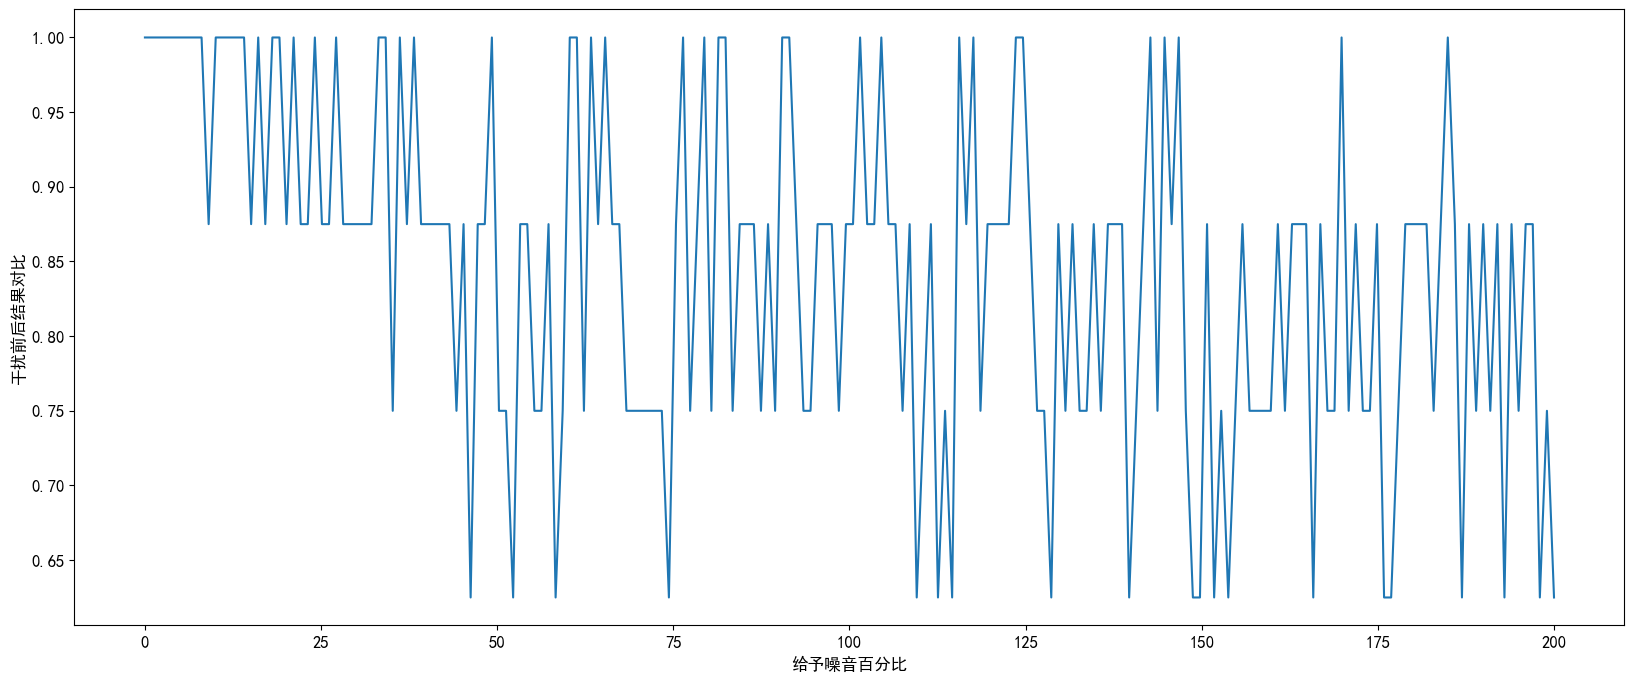
\includegraphics[width=0.7\textwidth]{21.png} %插入图片,[]中设置图片大小,{}中是图片文件名
	\caption{敏感性阈值图} %最终文档中希望显示的图片标题
	\label{Fig.main22} %用于文内引用的标签
\end{figure}

通过图21发现该模型的敏感性阈值d在(0,0.3)之间,模型的准确率都在85\%以上,当d在(0.3,0.45)之间模型的准确率都在75\%以上,而当d大于0.45时模型的准确率波动性大,预测准确率变化大,因此最好将数据的敏感性阈值控制在0.45以下。



% ------------------------------------------------------------ %
%    打开chapter文件夹里的问题四建模.tex文件,编辑其中的内容
% ------------------------------------------------------------ %
%    打开chapter文件夹里的问题四建模.tex文件,编辑其中的内容
% ------------------------------------------------------------ %
\section{问题四建模与求解}

为分析不同类别的玻璃样本的化学成分的关联关系,并比较它们之间关联关系的差异性,利用灰色关联性分析模型并比较它们之间的差异性,做出流程图如下:

\begin{figure}[H] 
	\centering %图片居中
	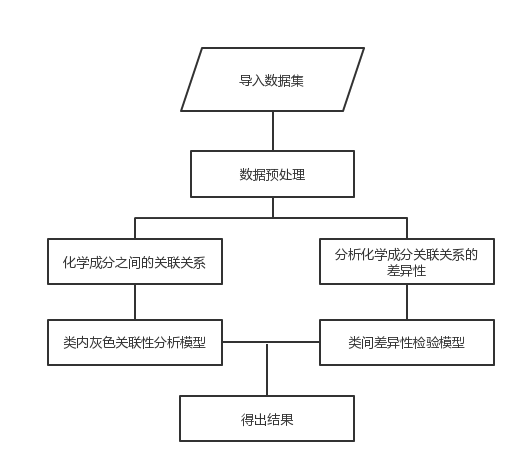
\includegraphics[width=0.7\textwidth]{22.png} %插入图片,[]中设置图片大小,{}中是图片文件名
	\caption{问题四流程图} %最终文档中希望显示的图片标题
	\label{Fig.main23} %用于文内引用的标签
\end{figure}


\subsection{数据预处理}

上述问题中处理后(补齐缺失值,删减异常值)的高钾玻璃数据表和铅钡玻璃数据表来进行类内的关联性分析,另外进行类间相关性分析。

\subsection{类内灰色关联性分析模型}

\subsubsection{模型准备}

对于类内各数据之间的关系,常见思路是进行相关系数矩求解,而求解相关性矩阵要进行正态性检验,本问对高钾玻璃和铅钡玻璃分别进行正态性检验,经过检验发现大部分特征都不满足正态分布(具体数据见附件)。因此,本问决定采用灰色关联预测进行关联性分析。

\subsubsection{模型建立}

对于灰色关联分析来分析类内的关联性,考虑到类内中每个化学成分之间都可能有关联性,因此用14个特征中随机抽取一个特征与其他特征进行灰色关联性分析。即有:

1. 将数据进行预处理:

\begin{equation}
    \widetilde{{{e}_{kj}}}=\frac{{{e}_{kj}}}{\overline{{{e}_{j}}}},\overline{{{e}_{j}}}=\frac{1}{{{n}_{z}}}\sum\limits_{k=1}^{n}{{{e}_{kj}}}(k=1,2,\cdots ,{{n}_{z}})
\end{equation}

\begin{equation}
    \widetilde{{{f}_{k}}}=\frac{{{f}_{k}}}{\overline{{{f}_{j}}}},\overline{{{f}_{j}}}=\frac{1}{{{n}_{z}}}\sum\limits_{k=1}^{n}{{{f}_{k}}}.
\end{equation}

2. 确定母序列和子序列:

\begin{equation}
    E={{\left[ {{e}_{1}},{{e}_{2}},\cdots ,{{e}_{13}} \right]}^{T}}.
\end{equation}

\begin{equation}
    F=\left[ \begin{matrix}
		{{f}_{11}} & {{f}_{12}} & \cdots  & {{f}_{1,13}}  \\
		{{f}_{21}} & {{f}_{22}} & \cdots  & {{f}_{2,13}}  \\
		\vdots  & \vdots  & \ddots  & \vdots   \\
		{{f}_{{{n}_{z}}1}} & {{f}_{{{n}_{z}}2}} & \cdots  & {{f}_{{{n}_{z}}13}}  \\
	\end{matrix} \right]
\end{equation}

3. 计算序列和母序列的关联系数:


\begin{equation}
    r=\underset{j}{\mathop{\min }}\,\underset{k}{\mathop{\min }}\,|{{f}_{0}}(k)-{{f}_{j}}(k)|
\end{equation}

\begin{equation}
    b=\underset{j}{\mathop{\max }}\,\underset{k}{\mathop{\max }}\,|{{f}_{0}}(k)-{{x}_{j}}(k)|
\end{equation}

4. 计算关联度:

(1)构造:

\begin{equation}
    {{a}_{k,q}}={{\xi }_{q}}(k)=\frac{r+\rho b}{|{{e}_{kq}}-{{f}_{q}}|+\rho b}.
\end{equation}

(2)计算关联度:

\begin{equation}
    R=\frac{1}{{{n}_{z}}}\sum\limits_{k=1}^{n}{{{\xi }_{q}}(k)}=\frac{1}{{{n}_{z}}}\sum\limits_{k=1}^{n}{{{a}_{kq}}}.
\end{equation}

\subsubsection{模型求解}

根据公式可以分别算出高钾与铅钡的类内的灰色关联结果(下表为高钾玻璃灰色关联结果,铅钡结果见附件)

\begin{figure}[H] 
	\centering %图片居中
	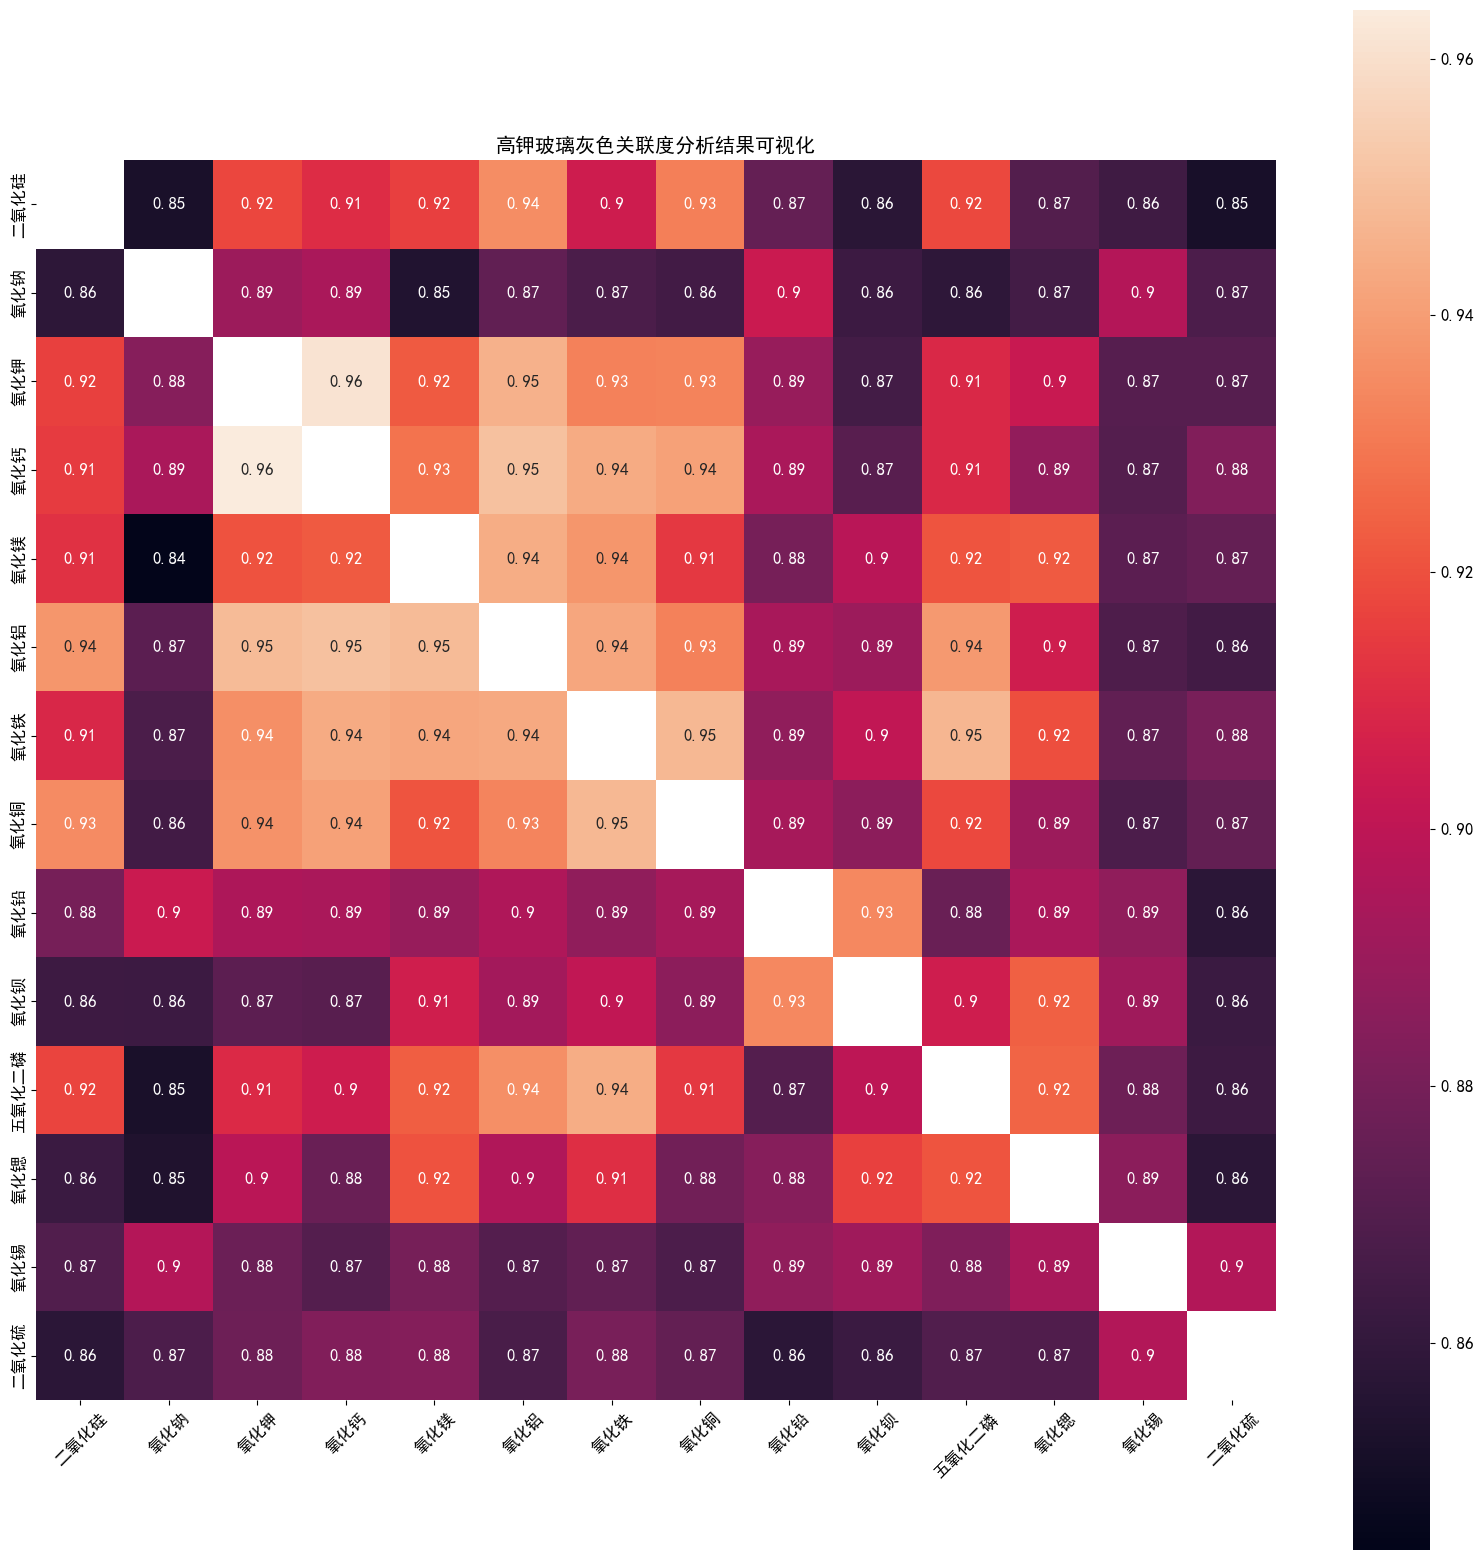
\includegraphics[width=0.7\textwidth]{23.png} %插入图片,[]中设置图片大小,{}中是图片文件名
	\caption{高钾玻璃关联度分析结果可视化图} %最终文档中希望显示的图片标题
	\label{Fig.main24} %用于文内引用的标签
\end{figure}

由图20可以看到每个化学成分之间的关联度结果最低为0.84,即整个类内的化学物质之间都存在的显著关联性,可以判断出在同类化学成分之间每种成分之间都存在关联关系。


\subsection{类间差异性检验模型}

\subsubsection{模型建立}

本问基于类内灰色关联得到的高钾类各化学成分与铅钡类化学成分的关联系数组成新的关联的系数表,需要对类间的同一化学成分关联性的差异性进行分析,配对t检验是一种用于配对定量数据之间的差异对比关系的优良检验方法。首先需要对两类数据进行正态性检验,检验之后发现都不满足正态分布。需要使用其他检验方法,因此使用非参数检验,本问所求两种类型同一化学成分的差异性可以采用非参数配对样本Wilcoxon符号秩检验进行检验。

\subsubsection{模型求解}

利用spasspro中的非参数检验配对样本Wilcoxon符号秩检验对于新表数据进行差异性检验,得出两类玻璃的同一化学物质的差异性显著系数表。

\begin{table}[H]
	\centering
	\begin{tabular}{c c c} 
		\toprule[1.5pt]
		化学成分 & 值(显著性) & Cohen's d值(差异幅度) \\
		\midrule[1pt]
		二氧化硅 & 0.116 & 0.427 \\
		氧化钠 & 0.221 & 0.23 \\
		氧化钾 & 0.101 & 0.373 \\
		氧化钙 & 0.600 & 0.139 \\
		氧化镁 & 0.507 & 0.088 \\
		氧化铝 & 0.753 & 0.013 \\
		氧化铁 & 0.087* & 0.359 \\
		氧化铜 & 0.807 & 0.059 \\
		氧化铅 & 0.013** & 0.727 \\
		氧化钡	& 0.016** &	0.625 \\
		五氧化二磷 & 0.507 & 0.033 \\
		氧化锶 & 0.064* & 0.453 \\
		氧化锡 & 0.116 & 0.209 \\
		二氧化硫 & 0.002*** & 0.56 \\
		\toprule[1.5pt]
\end{tabular}
\caption{差异性显著系数表}
\end{table}

由$p>0.05$可以判定上表两种类间化学成分中二氧化硅、氧化钠、氧化钾、氧化钙、氧化镁、氧化铝、氧化铁、氧化铜、五氧化二磷、氧化锶、氧化锡不能拒绝显著性假设,故两个量之间不存在显著性差异。

由$p\leq 0.5$可以判定上表两种类间化学成分中氧化铅、氧化钡、二氧化硫能拒绝显著性假设,故两个量之间存在显著性差异。

当两个变量之间具有显著性差异时,Cohen's d值一般都较大,说明两个变量之间有较大的差异幅度。




% ------------------------------------------------------------ %
%    打开chapter文件夹里的模型评价.tex文件,编辑其中的内容
% ------------------------------------------------------------ %
%    打开chapter文件夹里的模型评价.tex文件,编辑其中的内容
% ------------------------------------------------------------ %
\section{模型评价和改进}

\subsection{模型优点}

1. 在问题一中对文物表面是否风化与类型、颜色、纹饰关系分析过程中,不仅对于单变量之间进行了分析,还进一步用树模型进行了多变量与单变量的分析,同时利用互信息进一步对结果进行检验,提高模型的合理性。

2. 本文做了大量图表来统计分析数据特点,直观的对比出两类玻璃风化前后的化学成分的变化量以及各类玻璃化学成分之间的关系。

3. 在文本中多次对模型进行调参,利用混淆矩阵和多个指标检验,提高了模型的准确性。

4. 使用强分类器,构建Voting集成算法,得到一个完美模型,得到结果可信度高。

\subsection{模型缺点}

1. 做编码时由于颜色样本有7个非叙述类别,而数据集中存在大量的分类特征,没有找到合理高效的特征编码方式。

2. 本文在补充颜色缺失值时,鉴于分布分析补充黑色,而实际上在工业上常使用众数补充。

\subsection{模型改进}

在查阅文献时,涉猎了一种工业上常见新进的特征编码方式——目标编码,此方式通过计算类别出现的频率,对高维分类特征进行编码,避免出现维数灾难,同时也不会导致类别间的欧几里得距离过大。相信使用这种编码会让问题一中结果更具说服力。



% ------------------------------------------------------------ %
%    打开chapter文件夹里的参考文献.tex文件,编辑其中的内容
% ------------------------------------------------------------ %
%    打开chapter文件夹里的参考文献.tex文件,编辑其中的内容
% ------------------------------------------------------------ %
\section{参考文献}


% -------改下面的参考文献内容就行,别动这两句话!!!------- %
\renewcommand{\refname}{}
\vspace{-3em}  
% -------改下面的参考文献内容就行,别动这两句话!!!------- %


\begin{thebibliography}{50}  
	\bibitem{ref1}伏修锋,干福熹.基于多元统计分析方法对一批中国南方和西南地区的古玻璃成分的研究[J].文物保护与考古学2006(04).
	\bibitem{ref2}司守奎,孙玺菁.数学建模算法与应用(第3版)——北京:国防工业出版社,2021.4.
	\bibitem{ref3}周志华著;李楠译.集成学习:基础与算法——北京:电子工业出版社,2020.8. 
	\bibitem{ref4}司守奎,孙玺菁.Python数学建模算法与应用——北京:国防工业出版社,2022.1.
	\bibitem{ref5}王贺,刘鹏,钱乾著.机器学习算法竞赛实战——北京:人民邮电出版社,2021.9.
	\bibitem{ref6}何道江,黄旭东,张琼编.数学建模优秀论文选编——北京:科学出版社,2020.11.
	\bibitem{ref7}何伟,张良均主编.机器学习原理与实践——北京:人民邮电出版社,2021.7.
	\bibitem{ref8}孙玉林,余本国著.Python机器学习算法与实践——北京:电子工业出版社,2021,9.
\end{thebibliography} 


\end{document} 